%
%  Copyright (C) 2007
%  ASTRON (Netherlands Foundation for Research in Astronomy)
%  P.O.Box 2, 7990 AA Dwingeloo, The Netherlands, seg@astron.nl
%
%  $Id$
%
\documentclass[10pt]{lofar}
%
%% I prefer Bookman over Palatino, but I need Kerkis for math support
%\usepackage{bookman} 
\usepackage{mathpazo}      %% Palatino with matching math fonts.
\usepackage{amssymb}
\usepackage{layout}
\usepackage{color}
\usepackage{xspace}
\usepackage{url}           %% could also use package hyperref.
%\usepackage[colorlinks=false]{hyperref}
%
\newcounter{decision}
\newenvironment{decision}[1][Decision]{\begin{trivlist}\item[\hskip \labelsep {\bfseries #1 \refstepcounter{decision}\thedecision}]}{\end{trivlist}}
%
\newcommand{\todo}[1]{\begin{center}\fbox{\parbox{0.9\textwidth}{\textbf{!!TODO!! #1}}}\end{center}}
\newcommand{\cs}[1]{\textsc{cs}\begin{footnotesize}#1\end{footnotesize}\xspace}
\newcommand{\bbs}{\textsc{bbs}\xspace}
\newcommand{\lofar}{\textsc{lofar}\xspace}
\newcommand{\ms}{\textsc{ms}\xspace}
\newcommand{\me}{\textsc{me}\xspace}
\newcommand{\lsm}{\textsc{lsm}\xspace}
\newcommand{\aips}{\textsc{aips}\begin{footnotesize}++\end{footnotesize}\xspace}
\newcommand{\olap}{\textsc{olap}\xspace}
\newcommand{\meqtree}{\textsc{m}\begin{footnotesize}eq\end{footnotesize}\textsc{t}\begin{footnotesize}ree\end{footnotesize}\xspace}
%\newcommand{\meqtree}{MeqTree\xspace}
\newcommand{\predict}{\textsc{predict}\xspace}
\newcommand{\solve}{\textsc{solve}\xspace}
\newcommand{\subtract}{\textsc{subtract}\xspace}
\newcommand{\correct}{\textsc{correct}\xspace}
%
%
% Define the information of the page header
%
\renewcommand{\theAuthor}  {D.\ Hoogland}
\renewcommand{\theDOIssue} {2003-Jul-02}
\renewcommand{\theKOIssue} {Public}
\renewcommand{\theStatus}  {Draft}
\renewcommand{\theRevNR}   {0.1.1}
\renewcommand{\theScope}   {CEP}
\renewcommand{\theDocNR}   {LOFAR-ASTRON-DOC-xxx}
\renewcommand{\theFile}    {ftp://kant.astron.nl/pub/tex/lofar-cls-0.9.6.tgz}
%
% Define the title of the document
%

\renewcommand{\theTitle}
{Blackboard, a framework for imaging applications}

\renewcommand{\theTAuthor} {D.\ Hoogland}
%
% Define the names in the Verified table
%
\renewcommand{\theVNameList} {K.\ van der Schaaf\\
                              K.\ van der Schaaf}
\renewcommand{\theVSigList}  {o.p.v. \\
                              ......................................
                             }
\renewcommand{\theVDateList} {2003-Jul-02\\
                              .....................
                             }
\renewcommand{\theVRevList}  {0.1.0 \\
                              0.1.1 }
%
% Define the names in the Accepted table
%
\renewcommand{\theAHeada}    {Work Package Manager}
\renewcommand{\theAHeadb}    {System Engineering Manager}
\renewcommand{\theAHeadc}    {Program Manager}
\renewcommand{\theAManagera} {D.\ Hoogland}
\renewcommand{\theAManagerb} {K.\ van\ der\ Schaaf}
\renewcommand{\theAManagerc} {C.M.\ de\ Vos}
%
% This goes into the footer
%
\renewcommand{\theProject}   {LOFAR Project}
%
% Define the first,second and third columns of the distribution list
%
\renewcommand{\dGList} {%
                        ASTRON\\
                        \hspace{0.5cm} D.\ Hoogland\\
                        \hspace{0.5cm} K.\ van\ der\ Schaaf
                        \hspace{0.5cm} G.\  van Diepen\\
                        \hspace{0.5cm} A.\  van Gerdes\\
                        \hspace{0.5cm} J.\ Noordam
                       }
%
\renewcommand{\ddGList}{%
                        \\
                        J.\ Reitsma\\
                        O.\ Smirnov\\
                        C.M.\ de Vos
                       }
%
\renewcommand{\dOList}{%
                        ORDINA\\
                        \hspace{0.5cm} K-J.\ Wieringa\\[\baselineskip]
                        Snow B.V.\\
                        \hspace{0.5cm} D.\ Hoogland
}
%
% Define the version history
%
\renewcommand{\revList}     {%
                             0.0.1\\
                             0.1.0\\
                             0.1.1
                            }
\renewcommand{\dateList}    {%
                             2003-Jun-18\\
                             2003-Jun-24\\
                             2003-Jul-02
                            }
\renewcommand{\sectionList} {%
                             -\\
                             \ref{Sec2}\\
                             -
                            }
\renewcommand{\pageList}    {%
                             -\\
                             \pageref{Sec2}-\pageref{Sec2e}\\
                             -
                            }

\renewcommand{\changeList} {%
                            Creation in xml\\
                            rough sketch\\
                            Creation \LATEX version
                           }

%
\begin{document}
\maketitle
\newpage
%
\theDistributionList
\vspace{1cm}
\theDocumentRevision
\newpage
%
\begin{abstract}
\centering

\includegraphics[width=0.8\textwidth]{images/dt20070317}
\end{abstract}
\newpage
%
\tableofcontents
\newpage
%

\section{Introduction}
\label{sec:introduction}

\subsection{Purpose of This Document}
\label{subsec:purpose}
This document provides a detailed description of the architectural and
software design of the Blackboard Selfcal System (BBS) that will be used for
the calibration of the LOFAR observations. The primary goal of this document
is to provide information that is detailed enough to help the reader
understand the design considerations, choice of software architecture and
global design. We will not delve into the level of detailed software design,
since this will likely cause discrepancies between the actual code and this
document. For this level of detail, the reader is suggested to consult the
online code documentation. This document supersedes the previous version of
the BBS SDD~\cite{LOFAR-ASTRON-SDD-052}.

\subsection{Executive Summary}
\label{subsec:summary}

\subsection{Abbreviations}
\label{subsec:abbrev}
\begin{tabular}{@{}ll}
ACC   & Application Configuration and Control \\
BBS   & BlackBoard Selfcal system             \\
OLAP  & On-Line Appication Processing         \\
\end{tabular}

\cleardoublepage

\section{Architectural Design}
\label{sec:architectural-design}

\todo{see SDD-050 section 4.2 for requirements}

\subsection{Design Considerations}
\label{subsec:considerations}
The BlackBoard SelfCal (BBS) system is designed to do the calibration of LOFAR
in an efficient way. Although BBS is mainly developed for LOFAR, it may also
be used to calibrate other instruments as soon as their specific algorithms
are plugged in.

\subsubsection{Data Volume}
\label{subsubsec:data-volume}
The volume of the data coming from the LOFAR correlator is \emph{very} large.
During initial operation (mid 2008) the amount of data generated during an
average observation will be in the order of several terabytes. Once LOFAR is
fully operational, this number will have increased to almost a hundred
terabytes.  Given the output data rate of the correlator and the storage
capacity of harddisks, it is obvious that the data cannot be stored on a
single system, not even if an array of harddisks were used. The only feasible
way to handle these large data sets is to distribute them to multiple
computers. Each computer will have to store and manipulate part of the data.

\subsubsection{Distributed Processing}
\label{subsubsec:distributed-processing}

The Selfcal application will be running on the off-line and auxiliary
processing clusters of the central processing facility (see
\cite{LOFAR-ASTRON-ADD-012}). These clusters consist of Linux PCs in a high
bandwidth network. The BBS application will run on a large cluster, typically
consisting of several hundred nodes. Data stored in the CEP intermediate
storage facility will be distributed over multiple disks and will be accessed
by multiple nodes concurrently. Reordering tens of terabytes of data takes too
much time and should be avoided.  Therefore the data should be distributed
such that the various applications (e.g., calibration and imaging) can operate
well without reordering. The distribution should be such that large chunks of
data can be processed locally and only small amounts of data need to be sent
to other machines. There are a few axes along which the data may be
distributed:
\begin{description}
\item [Time] is probably not a good candidate, because a time slot contains a
lot of data (up to 0.7~GBytes during initial operation). This may lead to
problems in the online system when all data of a time slot are sent to a
single machine and written there. Another problem is that parallelization of
imaging gets hard because the data of all time slots have to be combined.
\item [Baseline] seems a better candidate, but will lead to imaging problems. 
This is because a single image needs data from different machines, so large
amounts of gridded or FFT-ed data have to be sent around.
\item [Frequency] seems to be the best candidate. Creating an image is usually
done per channel or for a few channels, so in principle the whole imaging
process can be done locally. It will result in an image cube distributed over
many machines, so the image display and analysis software have to be able to
handle this. The image cube can be very large (e.g., 256~GBytes for
1000~channels of $4000 \times 4000$ pixels for the 4~Stokes parameters). \\
Distribution in frequency means that, e.g., each subband is stored on a
separate machine.  If needed, each subband can be distributed further. Of
course, each machine should contain about the same amount of data to get good
load balancing. \\ 
Note that this distribution matches well with the way the
correlator and online system is designed.
\end{description}
The BBS calibration software is not dependent on a specific distribution, so
in the future other distributions can be used when applicable. However, it has
not been evaluated yet if that is also true for the imaging software.

\subsubsection{Scalable Architecture}
\label{subsubsec:scalable-architecture}
One important requirement is scalability. In order to avoid any performance
bottlenecks, unnecessary coupling between the different computing nodes should
be avoided as much as possible. When distributing data over frequency, we can
almost completely decouple the computing nodes, as we saw in the previous
section. Another way to reduce coupling is to make communication indirect as
well. Computing nodes should communicate through some kind of global shared
memory. There are several architectural patterns that describe this
approach. One of the oldest and best known is the Blackboard pattern, which we
will describe briefly below.

Computing nodes should communicate through some kind of global shared
memory. One obvious candidate for such shared memory is a database system. It
provides locking and notification (trigger) mechanisms, and sometimes even
command queueing. We have to be careful, though, that the database will not
become a bottleneck.

\subsection{Blackboard Pattern}
\label{subsec:blackboard}
The idea behind the Blackboard architecture is a collection of independent
processes that work cooperatively on a common data structure. Each program is
specialized in handling a particular part of the overall task, and all
programs work together on the solution. These specialized programs work
independent of each other. They do not call each other, nor is there a
predetermined sequence for their activation. Instead, the direction taken by
the system is mainly determined by the current state of progress. A central
control component evaluates the current state of processing and coordinates
the specialized programs. This data-directed control regime makes
experimentation with different algorithms possible, and allows experimentally
derived heuristics to control processing. This architecture is described in
\cite{Buschmann1996} and \cite{LOFAR-ASTRON-SDD-002}.

The Blackboard architecture is ideal for solving problems for which no
predetermined algorithm or solve strategy is known. However, for the design of
the BBS system, we've come to the conclusion that the operational system will
benefit in terms of performance when using a predefined solving strategy. The
"best" algorithm to perform a self-calibration run can be chosen from a
relatively short list of calibration strategies in advance (based, e.g., on
heuristics, or suggested by research done with the \meqtree system).  In fact,
the Shared Respository pattern~\cite{Lalanda1998}, which can be seen as a
generalization of the Blackboard pattern, is probably a better match for the
BBS system. It realizes indirect communication using a repository as shared
memory. Components put their output into memory that is accessible by other
components and retrieve their input from this shared memory (also called a
repository). Figure~\ref{fig:shared-repository-pattern} show the
specialization hierarchy of patterns based on the Shared Repository pattern.

\begin{figure}[!ht]
\centering
\fbox{
  \begin{picture}(440,110)(-20,-3)
  \footnotesize
  \thicklines
  \put(0,50){Shared Repository pattern}
  \put(100,61){\vector(2,1){40}}
  \put(100,53){\vector(1,0){40}}
  \put(100,45){\vector(2,-1){40}}
  \put(150,80){Controller pattern}
  \put(150,50){Blackboard pattern}
  \put(150,20){Repository Manager pattern}
  \put(230,57){\vector(3,1){40}}
  \put(230,49){\vector(3,-1){40}}
  \put(280,68){Blackboard-based Control pattern}
  \put(280,32){Hierarchical Blackboard pattern}
  \end{picture}
}
\caption{Patterns based on the Shared Repository pattern, after
Lalanda~\cite{Lalanda1998}.}
\label{fig:shared-repository-pattern}
\end{figure}

\begin{description}
\item [Controller pattern] introduces a control component in the system, which
rules the system and schedules activation of other components. This pattern
can be applied to deterministic problems where sequences of components
activation can be determined off-line and coded in the controller using
various techniques.
\item[Repository Manager pattern] is applicabe in a distributed
environment. It introduces a repository manager which sends notification of
data creation or modification to the software components.
\item[Blackboard pattern] refines the Controller pattern to deal with
non-deterministic problems.
\end{description}

For BBS, we will need a global controller, which could be implemented using
the Controller pattern; and a notification or trigger mechanism to inform the
computing nodes of changes to the shared memory, which could be implemented
using the Repository Manager pattern. The shared memory is used as the common
knowledge base for the self-calibration process, and will be implemented as a
database. Using a database system has the advantage that locking, notification
(trigger) and sometimes even command queueing mechanisms are provided
out-of-the-box.

The database will be separated into two parts. One part, the Command Queue,
will contain a list of commands (or work orders) to be sent to each computing
node. The other part, the Parameter Solutions database, will contain the
values and quality of the (partial) solutions calculated by each computing
node. The database can be used as an external source for various assessments
of the solutions.

\cleardoublepage

\section{System Overview}
\label{sec:overview}

\subsection{Subsystems}
\label{subsec:subsystems}
BBS is split into two parts. BBS Control takes care of the distributed
processing by means of the Blackboard pattern. BBS Kernel does the actual
processing; it executes a series of steps where each step consists of an
operation like solve or correct.


\subsubsection{BBS Control}
\label{subsubsec:sys-control}

The BBS Control subsystem is responsible for controlling the execution of a
self calibration strategy. A strategy consists of an ordered list of commands,
which will be executed by the BBS Kernel subsystem.

The key idea is that a subset of the data (the so-called \emph{work domain})
is kept in memory; as many commands as possible are executed on these data
before the next data chunk is accessed. A strategy defines the size of the
work domain (in time and frequency) and optionally which stations and
correlations are contained in the work domain. It is also possible to define
an integration interval in time and frequency to achieve that, say, a longer
time interval can be used. The basic concept is that on each machine the data
contained in the work domain have to fit in memory. The BBS Kernel iterates
over the work domains to process all the data.  For each strategy a number of
steps can be defined. For instance, when peeling 10 Cat I sources, at least 30
steps can be defined. For each source, step~1 is solving for the gain in the
direction of the source, step~2 is subtracting the source, and step~3 shifts
to the next source. Note that only after the last subtraction the residual
data need to be written.  In this way the data are read and/or written only
once per strategy.

\begin{figure}[!ht]
\centering
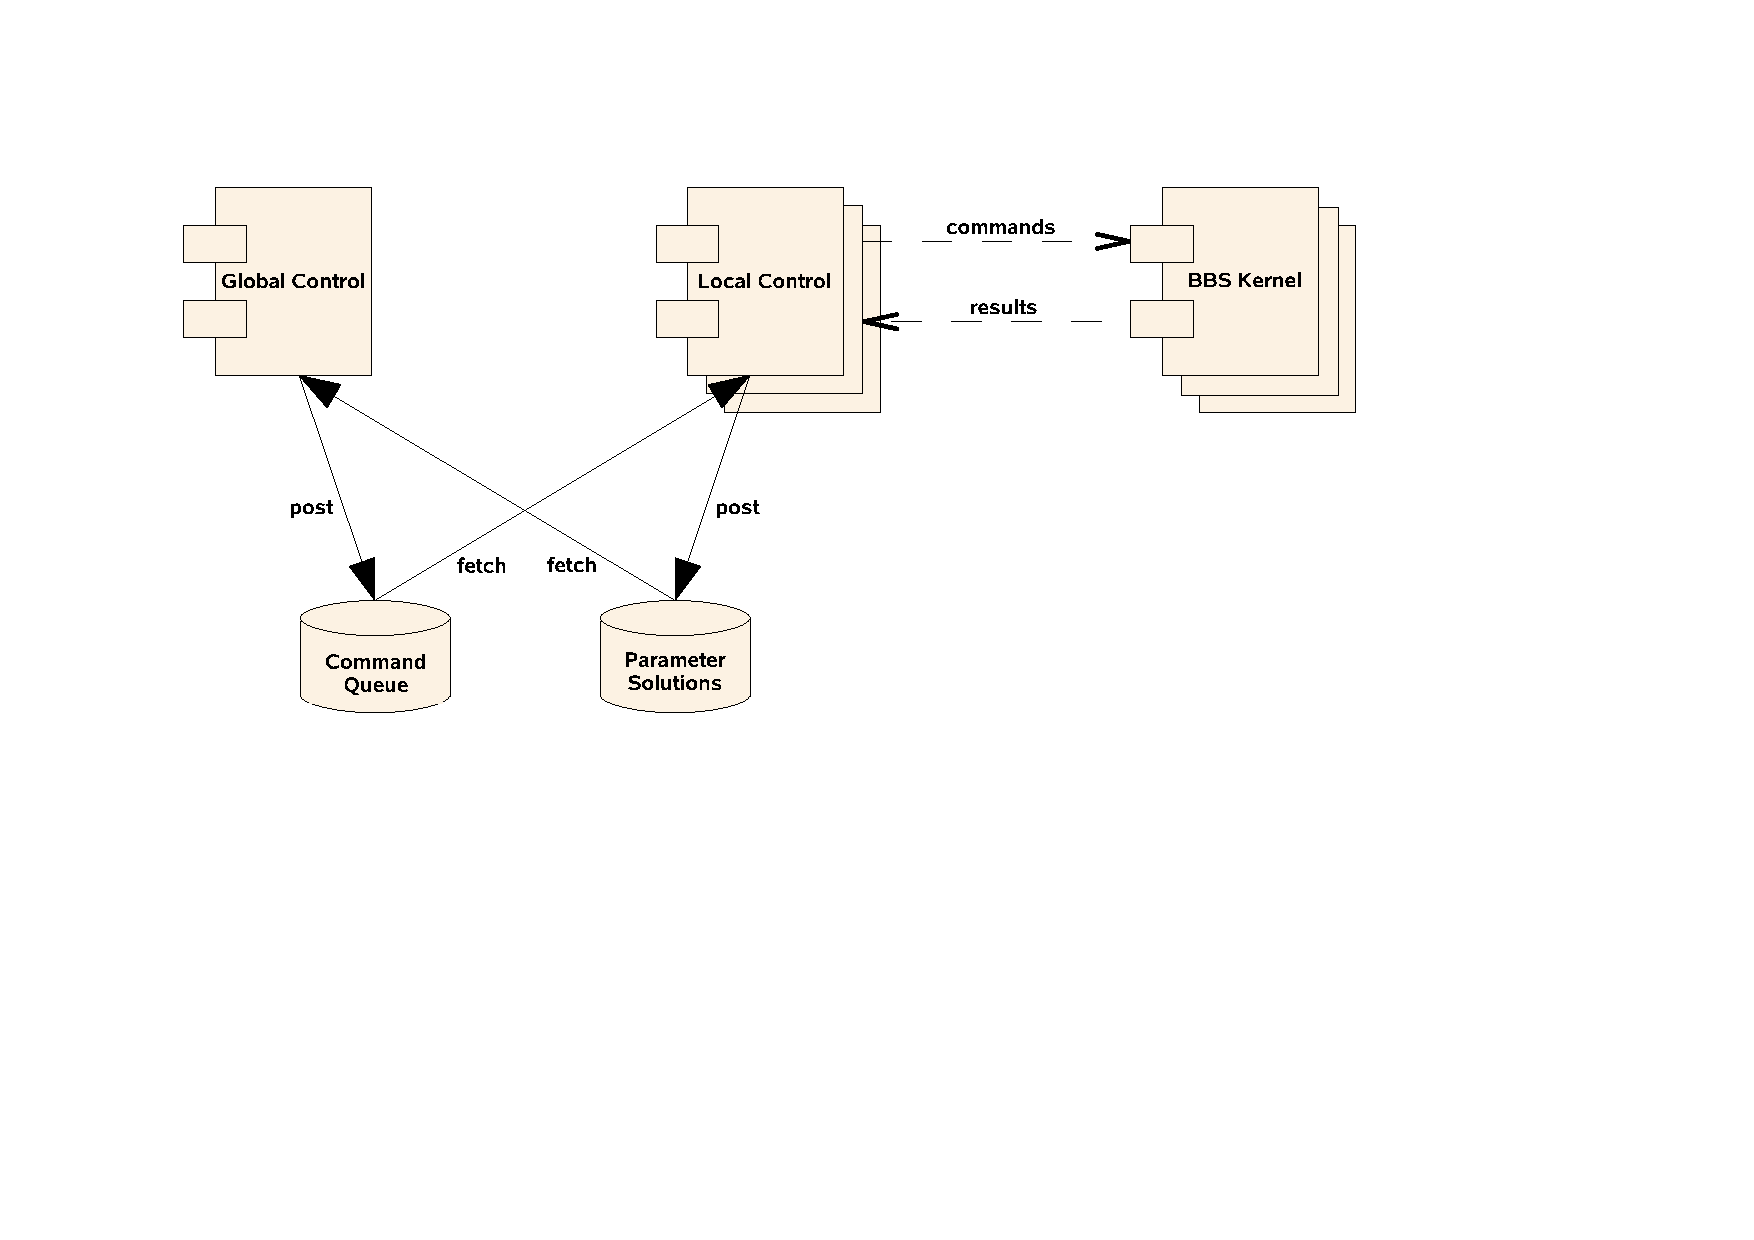
\includegraphics[width=0.6\textwidth]{images/bbs-control-global-design}
\caption{Global design of the BBS Control system. Global Control posts
commands to the Command Queue. These commands are asynchronously retrieved by
Local Control and forwarded to the BBS Kernel. After execution of the command,
BBS Kernel returns the result to Local Control, which in turn posts it to the
Parameter Solutions database. Global Control checks the quality of these
solutions and takes appropriate action.}
\label{fig:bbs-control-global-design}
\end{figure}

The calibration process is controlled by the BBS Control
subsystem. Figure~\ref{fig:bbs-control-global-design} depicts the general
control structure. The BBS Control subsystem consists of one global
controller, which acts as the main process, and multiple local controllers,
each controlling one BBS Kernel subsystem. The global controller posts one or
more commands (steps) to the Command Queue. Each local controller fetches the
next command from the Command Queue and forwards the command to the BBS Kernel
subsystem. The kernel returns parameter solutions and their quality metrics to
the local controller, which, in turn, posts the results to the Parameter
Solutions database. The global controller inspects the results and decides
which action should be taken next.

Since all communication takes places via the Blackboard, there is no need for
a direct connection between the BBS Control and the BBS Kernel subsystems.
The Blackboard contains all the relevant information about the current state
of the self calibration process. This information can be used by other
(external) processes to monitor the calibration process and to plot results.
See~\cite{LOFAR-ASTRON-SDD-002} for more details on the Blackboard
architecture and roles of the controller.


\subsubsection{BBS Kernel}
\label{subsubsec:sys-kernel}

\subsubsection{BBS Database}
\label{subsubsec:sys-database}

\subsection{Interfaces}
\label{subsec:sys-interfaces}

\subsubsection{Context Diagram}
\label{subsubsec:context}
The BlackBoard Selfcal system interfaces with several other components. The context of BBS is shown in figure~\ref{fig:bbs-context-diagram}.

\begin{figure}[!ht]
\centering
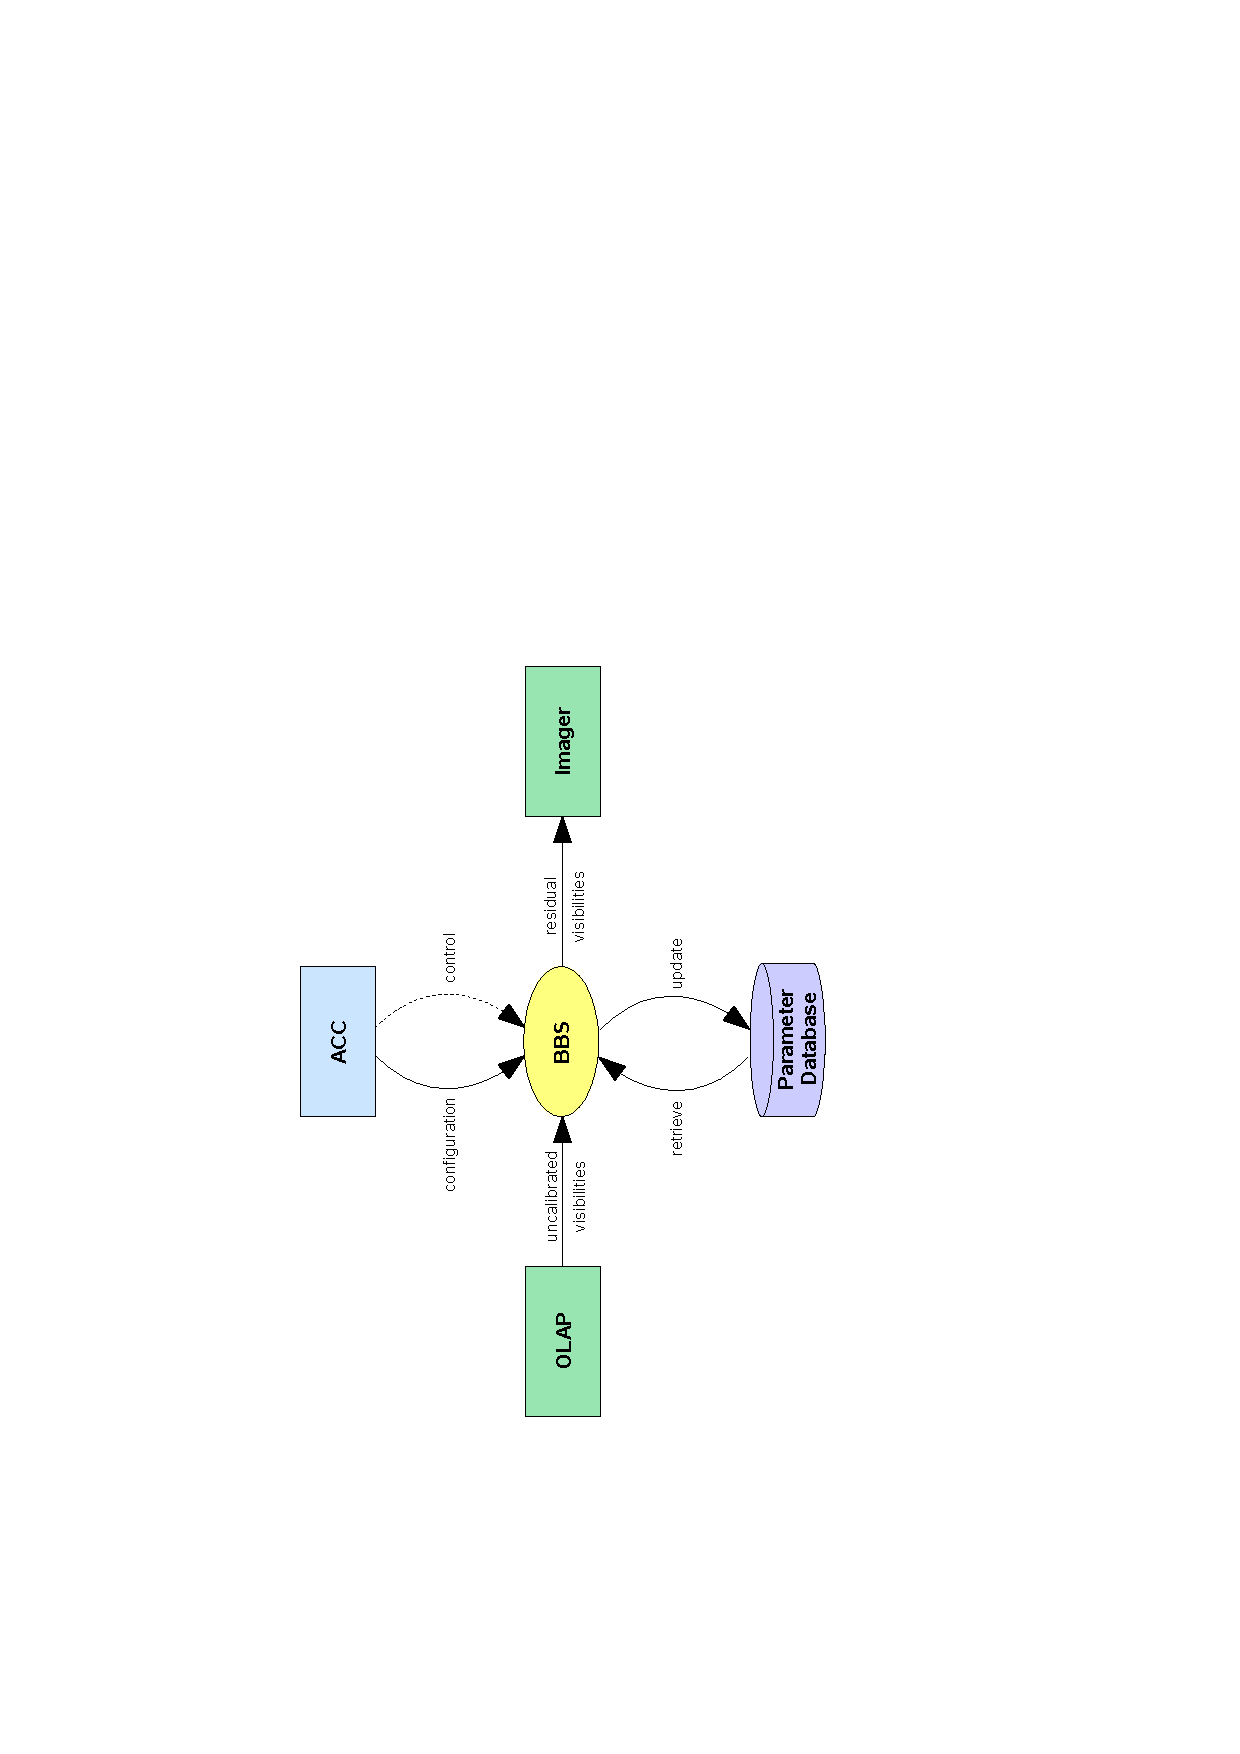
\includegraphics[width=0.5\textwidth,angle=-90]{images/bbs-context-diagram}
\caption{Context diagram for the BlackBoard Selfcal system. OLAP supplies the
input data, which are stored as a Measurement Set. ACC configures and controls
BBS. The Parameter Database
%---consisting of an Instrument Model, a Local Sky Model, and a Minimal Ionospheric Model---
is both read and updated by BBS.}
\label{fig:bbs-context-diagram}
\end{figure}

\begin{description}
\item [ACC] configures and controls BBS. Configuration is done using a so-called \emph{parset} file, which is generated by ACC prior to starting the BBS appications. Each BBS applications reads, during initiaization, its \emph{parset} file, containing a number of key-value pairs that set several run-time configuration parameters of the applications. All BBS applications implement the control interface that is provided by ACC~\cite{LOFAR-ASTRON-SDD-037}, which enables ACC to control these applications.
\item [OLAP] stores the observational data as visibilities into one more Measurement Sets
\item [Imager]
\item [Parameter database]
\end{description}

\subsubsection{BBS Control}
\label{subsubsec:interf-control}

\begin{itemize}
\item ACC
\item Command Queue
\item Parameter database
\end{itemize}

\subsubsection{BBS Kernel}
\label{subsubsec:interf-kernel}

\begin{itemize}
\item MS
\item ParmDB and LSM
\item ACC
\item kernel -- solver
\item kernel -- black board
\end{itemize}

\subsubsection{BBS Database}
\label{subsubsec:interf-database}

\cleardoublepage

\section{Software Design}
\label{sec:software-design}

\subsection{Terminology}
\label{subsec:terminology}

\subsubsection{Domains}
\label{subsubsec:domains}
A central concept in \bbs is the \emph{domain}: A 2-D rectangular region in
$frequency$ and $time$. In table \ref{tab:domains} we define seven different
domain types that are useful for discussing the design of \bbs. Figure
\ref{fig:domains} illustrates the different domain types and how they relate to
each other.

\begin{table}[htb!]
\centering
\begin{tabular}{lp{0.60\textwidth}}
\hline
\textbf{Name} & \textbf{Description}\\
\hline
\texttt{data domain} & The domain covered by a single observation\\
\hline
\texttt{local data domain} & Part of the data domain that is local to (i.e.
stored at) a given compute node\\
\hline
\texttt{work domain} & Part of the data domain which is processed together\\
\hline
\texttt{local work domain} & Intersection of the work domain and the local data
domain (should fit in the node's main memory)\\
\hline
\texttt{solve domain} & Part of the data domain that is used to solve for a set
of unknowns\\
\hline
\texttt{local solve domain} & A solve domain that \emph{intersects} the local
data domain\\
\hline
\texttt{validity domain} & Domain on which a \emph{funklet} is considered
valid\\
\end{tabular}
\caption{An overview of the domain types used in \bbs.}
\label{tab:domains}
\end{table}

\subsubsection{Models, parameters, funklets, and coefficients} 
\label{subsubsec:models-parameters-funklets-coefficients}
Self calibration revolves around fitting a \emph{model} to the observed data by
adjusting the parameters of the model. On the coarsest scale a model for the
calibration of \lofar describes the instrument, the environment, and the sky.
This model can be decomposed into smaller (sub)models, such as a model for the
beamshape, the bandpass, or the ionosphere (see also \cite[sec.
2]{LOFAR-ASTRON-SDD-050}).

\todo{ref Hamaker, aips++ note of Jan N.}

In general, a \emph{parameter} can be a constant or a continuous function of one
or more variables such as $frequency$, $time$, and $direction$.

The value of a parameter is represented by a set of \emph{funklets}. A funklet
is an approximation of the value of a parameter on a bounded domain, termed
\emph{validity domain}. Figure \ref{fig:funklet} illustrates the relation
between parameters and funklets.

A commonly used type of funklet is a polynomial of arbitrary degree in
$frequency$ and/or $time$. Other posibilities include Fourier series expansions,
shapelets, and splines.

\begin{figure}[htbp]
\centering
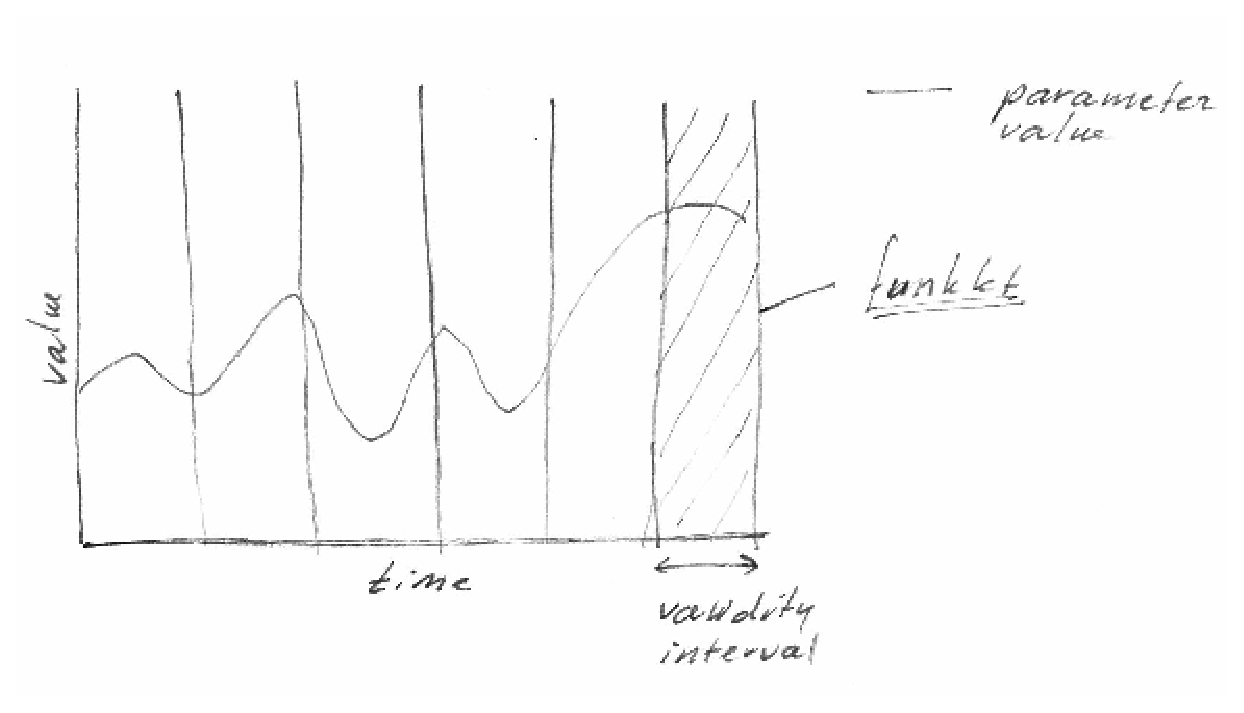
\includegraphics[width=0.75\textwidth]{images/funklet.eps}
\caption{This figure shows a set of funklets with associated validity domains
that together represent the value of a parameter on a larger domain.}
\label{fig:funklet}
\end{figure}

Validity domains and solve domains are related concepts. The validity domain of
a funklet equals the solve domain used to fit the coefficients of the funklet.
For example, suppose we try to fit a parameter
\texttt{gain:11:phase:CS10}\footnote{The phase of element $g_{11}$ of the $2
\times 2$ diagonal G-jones matrix of station CS10.} using $0^{th}$-degree
polynomials and a solve domain size of a single channel width times 5
integration periods. The solve domain size defines a grid of solve domains on
the work domain (see figure~\ref{fig:domains}). For each solve domain a funklet
exists with a matching validity domain that represents the value of parameter
\texttt{gain:11:phase:CS10} on that domain. To fit the coefficients of a funklet
we need the values of other parameters as well. The validity domains of the
funklets that represent these parameters will most likely be different, because
they were fitted at some earlier time using potentially different solve domains.
In summary: The validity domain of a funklet determines in what region the value
of the funklet is considered valid; A solve domain determines which part of the
observed data is used to fit the is used to fit the coefficients of a funklet.

The problem of fitting a parameter can now be restated as fitting the
coefficients of a \emph{set} of funklets defined on a set of non-overlapping
solve domains.

\subsection{Distribution}
\label{subsec:distribution}

The unit of work for most operations (i.e. \predict, \subtract, \correct) is a
single complex visibility. These operations are embarrassingly parallel:
communication between nodes is not necessary.

The only operation that is not guaranteed to be embarrassingly parallel is the
\solve operation. The unit of work for this operation is a single solve domain.
As long as every solve domain is completely contained within the local data
domain of a node, the \solve operation can be performed locally. However, if a
solve domain intersects the local data domains of multiple nodes, communication
between these nodes becomes necessary.

\subsubsection{Data distribution}
\label{subsubsec:distribution-data}
Figure \ref{fig:domains} shows how the data is typically distributed over the
compute nodes. The visibility data computed by the correlator is distributed
according to frequency, as is shown in the figure. Visibility data may be
unavailable, because the subbands recorded during an observation are not
required to be consecutive. All \emph{available} data is distributed equally
over the nodes. 

\begin{figure}[htbp]
\centering
%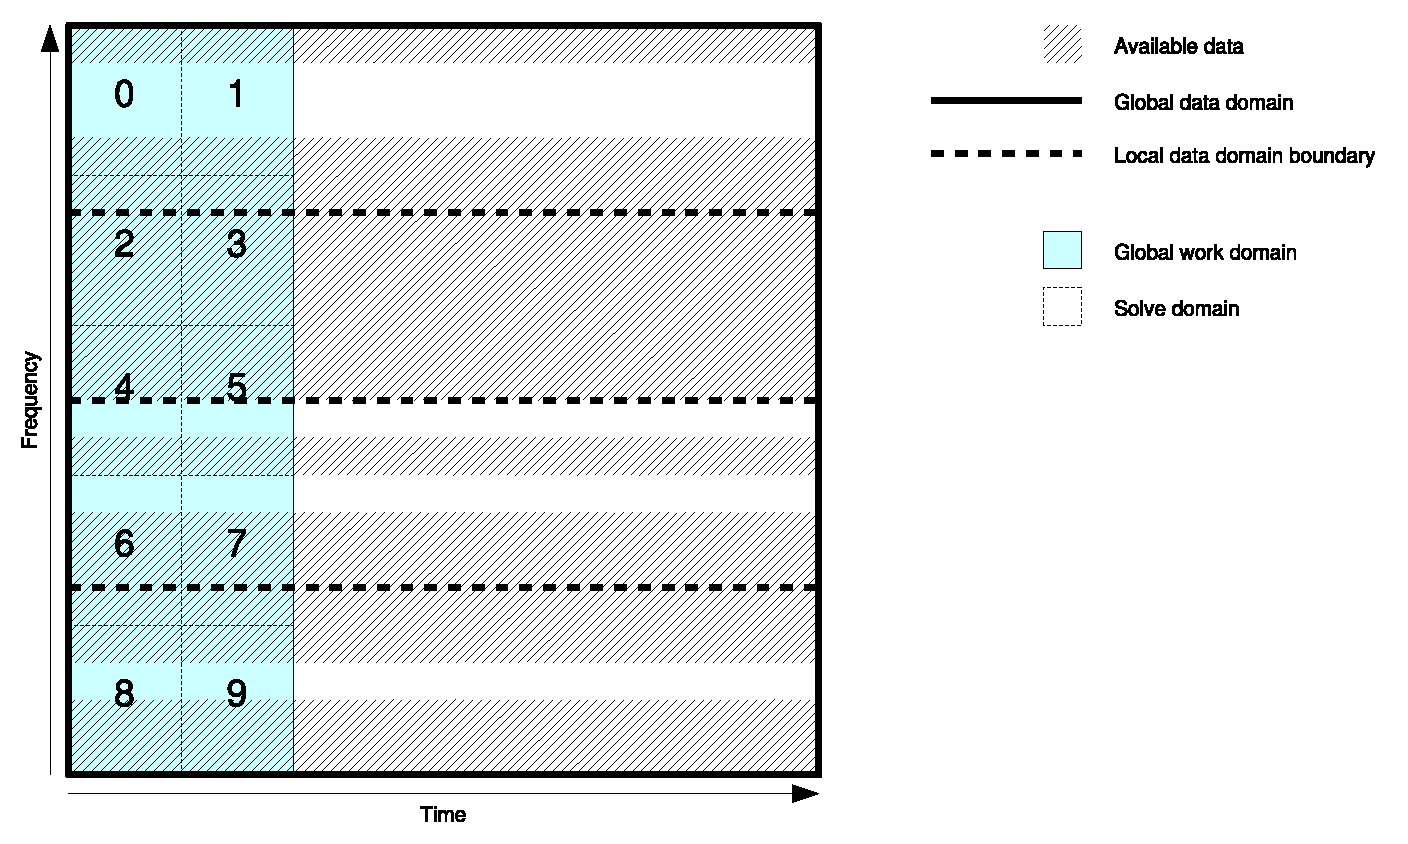
\includegraphics[scale=0.5]{images/domains.ps}
\includegraphics[scale=0.5]{images/solve_domains.ps}
\caption{Data distribution and partitioning of the work domain into solve
domains during a \solve operation. See Table~\ref{tab:domains} for the definition
of the different domain types.}
\label{fig:domains}
\end{figure}

The size of the work domain is specified by the user. It should be chosen such
that each node can read its local work domain into main memory. Thus, all steps
of the calibration \emph{strategy} can be executed on the work domain without
having to read data more than once. After the work domain has been processed,
the global controller instructs the local controllers to continue with the next
chunk of data.

During execution of a \solve operations, the work domain is partitioned into
solve domains based on a user specified solve domain size.
Figure~\ref{fig:solve_domains} shows an example where the work domain is
partitioned into ten separate solve domains. Six solve domains are entrirely
local: solve domains 0, 1, 4, 5, 8, and 9. The other solve domains span multiple
nodes.

%\begin{figure}[htbp]
%\centering
%\includegraphics[scale=0.5]{images/solve_domains.ps}
%\caption{Partitioning of the work domain into solve domains during a \solve
%operation.}
%\label{fig:solve_domains}
%\end{figure}

\paragraph{Solve domain size}

Because the local work domain is determined by the intersection of the work
domain and the local data domain, and the visibility data is distributed in
frequency, the work domain has to span the \emph{entire} frequency axis to keep
all the nodes busy. This implies that the largest possible size of the local
work domain \emph{in time} is more limited than necessary.

The largest possible \emph{area} (channels $\times$ integration periods) of the
local work domain is (assuming 77 stations, 8\textsc{gb} of local memory):

\[
area=\frac{8\cdot2^{30}\;bytes}{\frac{1}{2}\times(77 \times 76) \; interf.
\times 4 \; correlations \times 8 \; bytes/correlation} \approx 85441
\]

However, due to the way the work domain is defined, the largest possible size in
time is limited to the area divided by the number of channels stored per node.
Assuming 32000 channels and a cluster of 500 nodes:

\[
time=\frac{85441}{32000\;channels \div 500\;nodes} \approx 1335\;integration\;
periods
\]

It is currently an open question if this limit is within requirements. This will
depend on the type of \solve operations the user wants to perform.

\paragraph{Solve domain truncation}

If the size of the work domain along any dimension is not an integer multiple of
the specfied solve domain size, the solve domains at the boundaries will get
truncated. 

It is currently an open question if solve domain trunction is acceptable or not.
In principle, the work domain size could be adjusted automatically to avoid
solve domain truncation. This is not completely trivial, because a strategy can
contain multiple solve steps each of which can have a different solve domain
size.

Because \emph{all} steps of a strategy are executed on the work domain, the size
of the work domain must be an integer multiple of the size of each of the
specified solve domain sizes to completely avoid truncation. Assuming the
size of the work domain is specified in, or converted to, integers (or
fractional numbers), e.g. number of channels times number of integration
periods, the size of the work domain should be set to a multiple of the least
common multiple of the different solve domain sizes.

\subsubsection{Communication}
\label{subsubsec:distribution-communication}

Figure~\ref{fig:distribution-communication} shows the communication paths used
in \bbs. The blackboard is essentially used as \emph{shared memory} that retains
the state of the (distributed) calibration process. Shared memory allows
decoupling of the global controller and the local controllers, and easy
monitoring by external tools.

\begin{figure}[htb!]
\centering
\includegraphics[width=0.7\textwidth]{images/communication.ps}
\caption{Overview of the communication paths used in \bbs.}
\label{fig:distribution-communication}
\end{figure}

A potential risk of this design is that the shared memory becomes a performance
bottleneck.  All local controllers need to access the shared memory and this
access will typically be (quasi-) concurrent, because all local controllers
perform the same operations on approximately equal amounts of data. A related
concern, raised in \cite[p.19]{LOFAR-ASTRON-SDD-052}, is that local controllers
may have to poll the shared memory to check for updates. This depends on the
implementation of the shared memory component. Most modern databases, for
instance, support asynchronous notification of client processes thus avoiding
the need for polling. Performance tests should be carried out in the near future
to asses if the design meets the requirements.

Figure~\ref{fig:distribution-communication} shows that there is a direct link
between the local controller and the solver. One could wonder why the
communication is not routed via the shared memory. There are two reasons for
this. First, exchanging information between local controllers and solvers via
shared memory imposes unnecessary synchronisation. To fit the funklets defined
on a given solve domain, information about that solve domains needs only to be
exchanged between the local controller(s) \emph{that share the solve domain} and
a solver. Second, the amount of data that needs to be communicated from a local
controller to a solver is considerable and encoded in a form that is unsuitable
for monitoring.

The updated coefficients communicated from a solver to the relevant local
controllers \emph{are} suitable for monitoring. Of course, using direct
communication between kernel and solver does not prohibit writing the updated
coefficients to shared memory as well. Assuming monitoring coefficient values
during iteration is primarily used for debugging purposes, this is probably
acceptable.

At the start of a \solve operation a solver needs the initial values of the
funklet coefficients for the solve domains it will process. At the end of the
\solve operations the updated coefficient values have to be written to shared
memory. (If monitoring coefficient values during iteration is required, the
updated coefficients need to be written after each iteration as well.)

In the current design the local controller sends the initial coefficient values
to the solver and writes the updated coefficients to shared memory. Thus, the
design of the solver component can be kept simple. Yet it also implies that the
updated coefficient values of solve domains that are shared between multiple
nodes will be written multiple times. This is not a problem from a data
consistency point of view, but may aversely affect performance. Multiple writes
could be avoided if the solver is made responsible for updating the shared
memory.

\subsection{BBS Control}
\label{subsec:design-control}

\subsubsection{BBS Strategy}
\label{subsubsec:design-strategy}
One iteration in the so-called \emph{Major 
Cycle}~\cite[sec.~4.1]{LOFAR-ASTRON-SDD-050} can be described by a BBS
Strategy. A strategy defines a relationship between the data set of a given
observation, which is stored in a Measurement Set, and the parameter database
holding (intermediate) values of the model parameters that will be estimated
as part of the self calibration process. At least two models are used in the
current self calibration setup: the Local Sky Model (LSM) and the Instrument
Model. The Data Selection associated with a BBS Strategy defines the selection
of the observed data that will be used for the complete strategy. Here you
can, for example, specify which frequency bands, time intervals, and baselines
should be used during this self calibration run. A strategy is defined in
terms of one or more BBS Steps (see section~\ref{subsubsec:design-step}
below).

\begin{figure}[!ht]
\centering
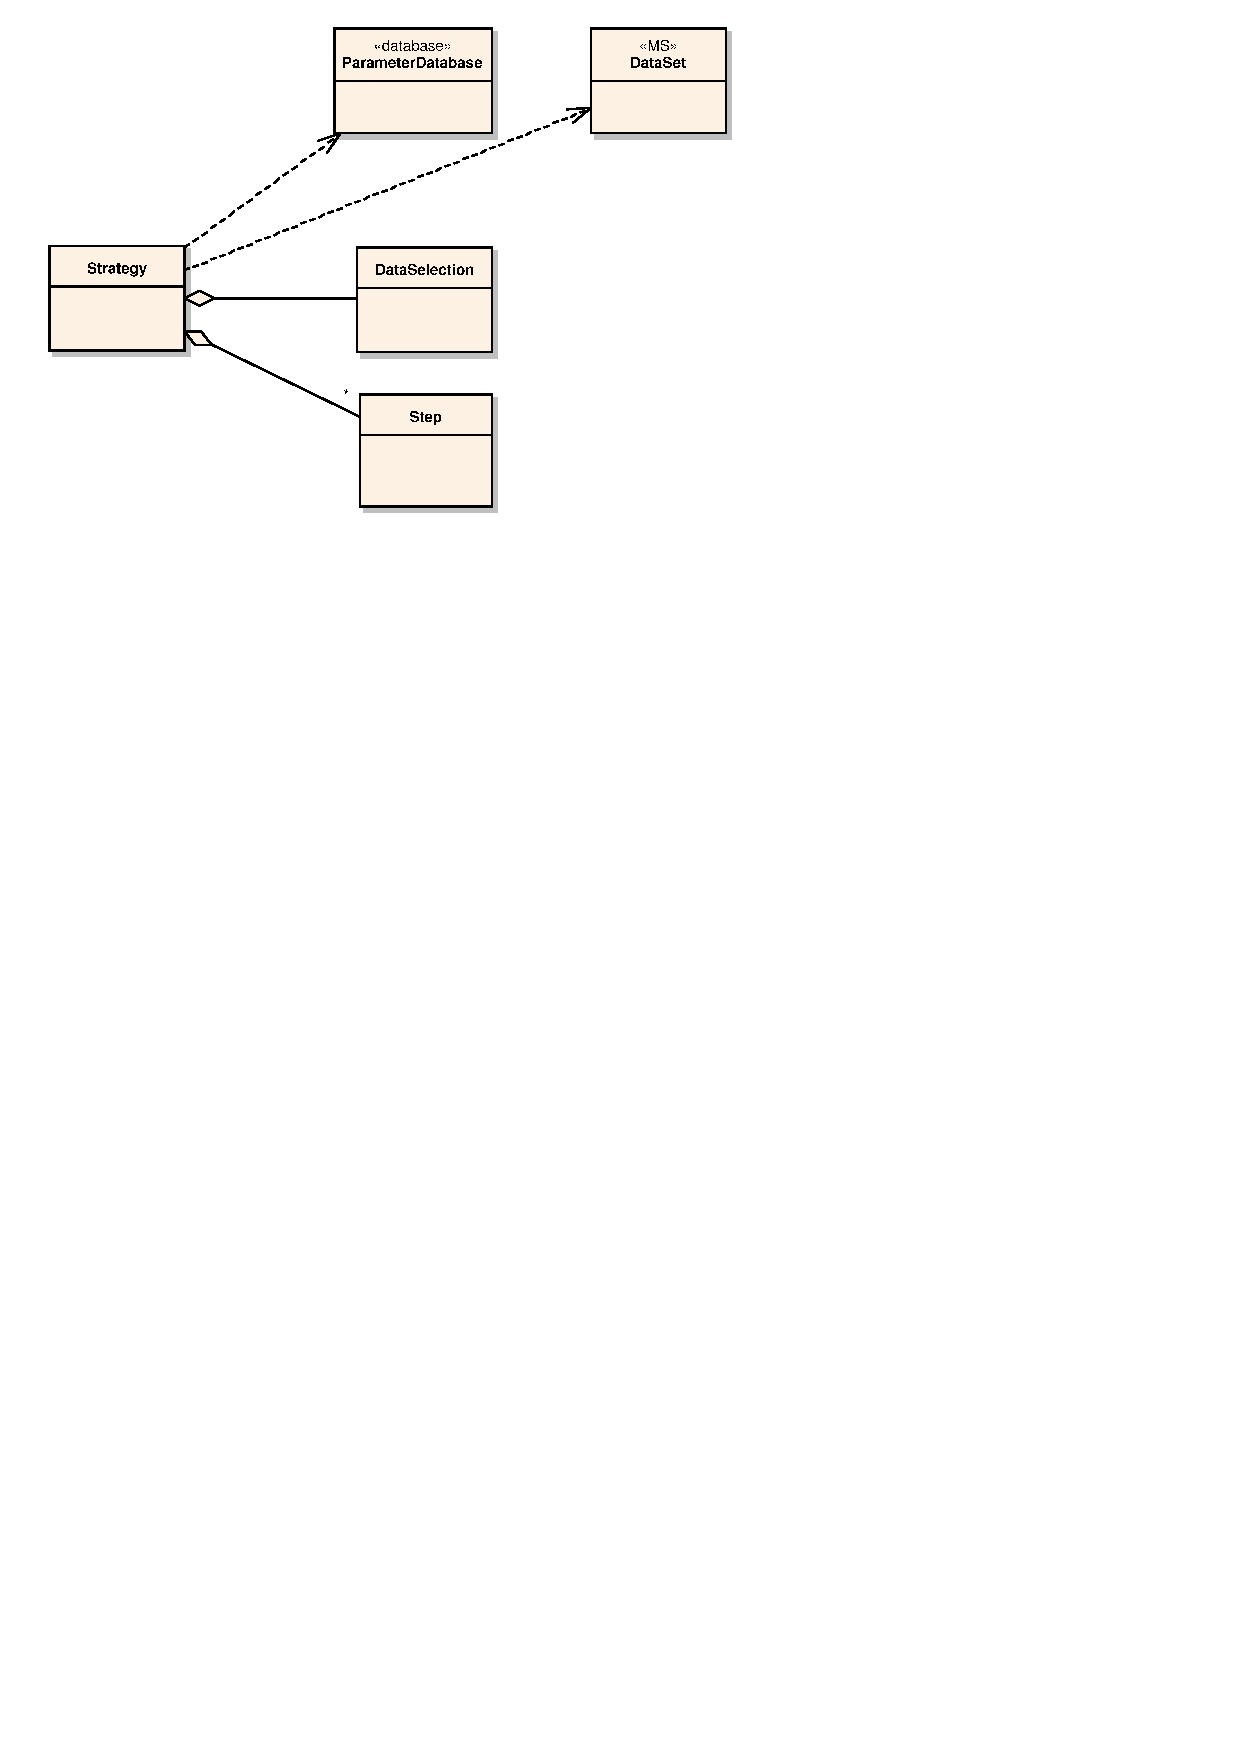
\includegraphics[width=0.5\textwidth]{images/bbs-strategy-class-diagram}
\caption{The BBS Strategy class defines the strategy to be used for the
current self calibration run.}
\label{fig:bbsstrategy}
\end{figure}

\subsubsection{BBS Step}
\label{subsubsec:design-step}
%A BBS Strategy is defined in terms of one or more BBS Steps. 
The BBS Step class is designed as a Composite pattern~\cite{Gamma1995}, which means that
each BBS Step can itself be made up of one or more BBS Steps. The Composite
pattern provides an easy way to define a tree-like structure. Leaf classes,
like SolveStep cannot be further subdivided; they describe one single
piece of work that can be handed over to the BBS Kernel. Currently, there is a
total of seven leaf classes, each defining one single piece of work.

\begin{figure}[!ht]
\centering
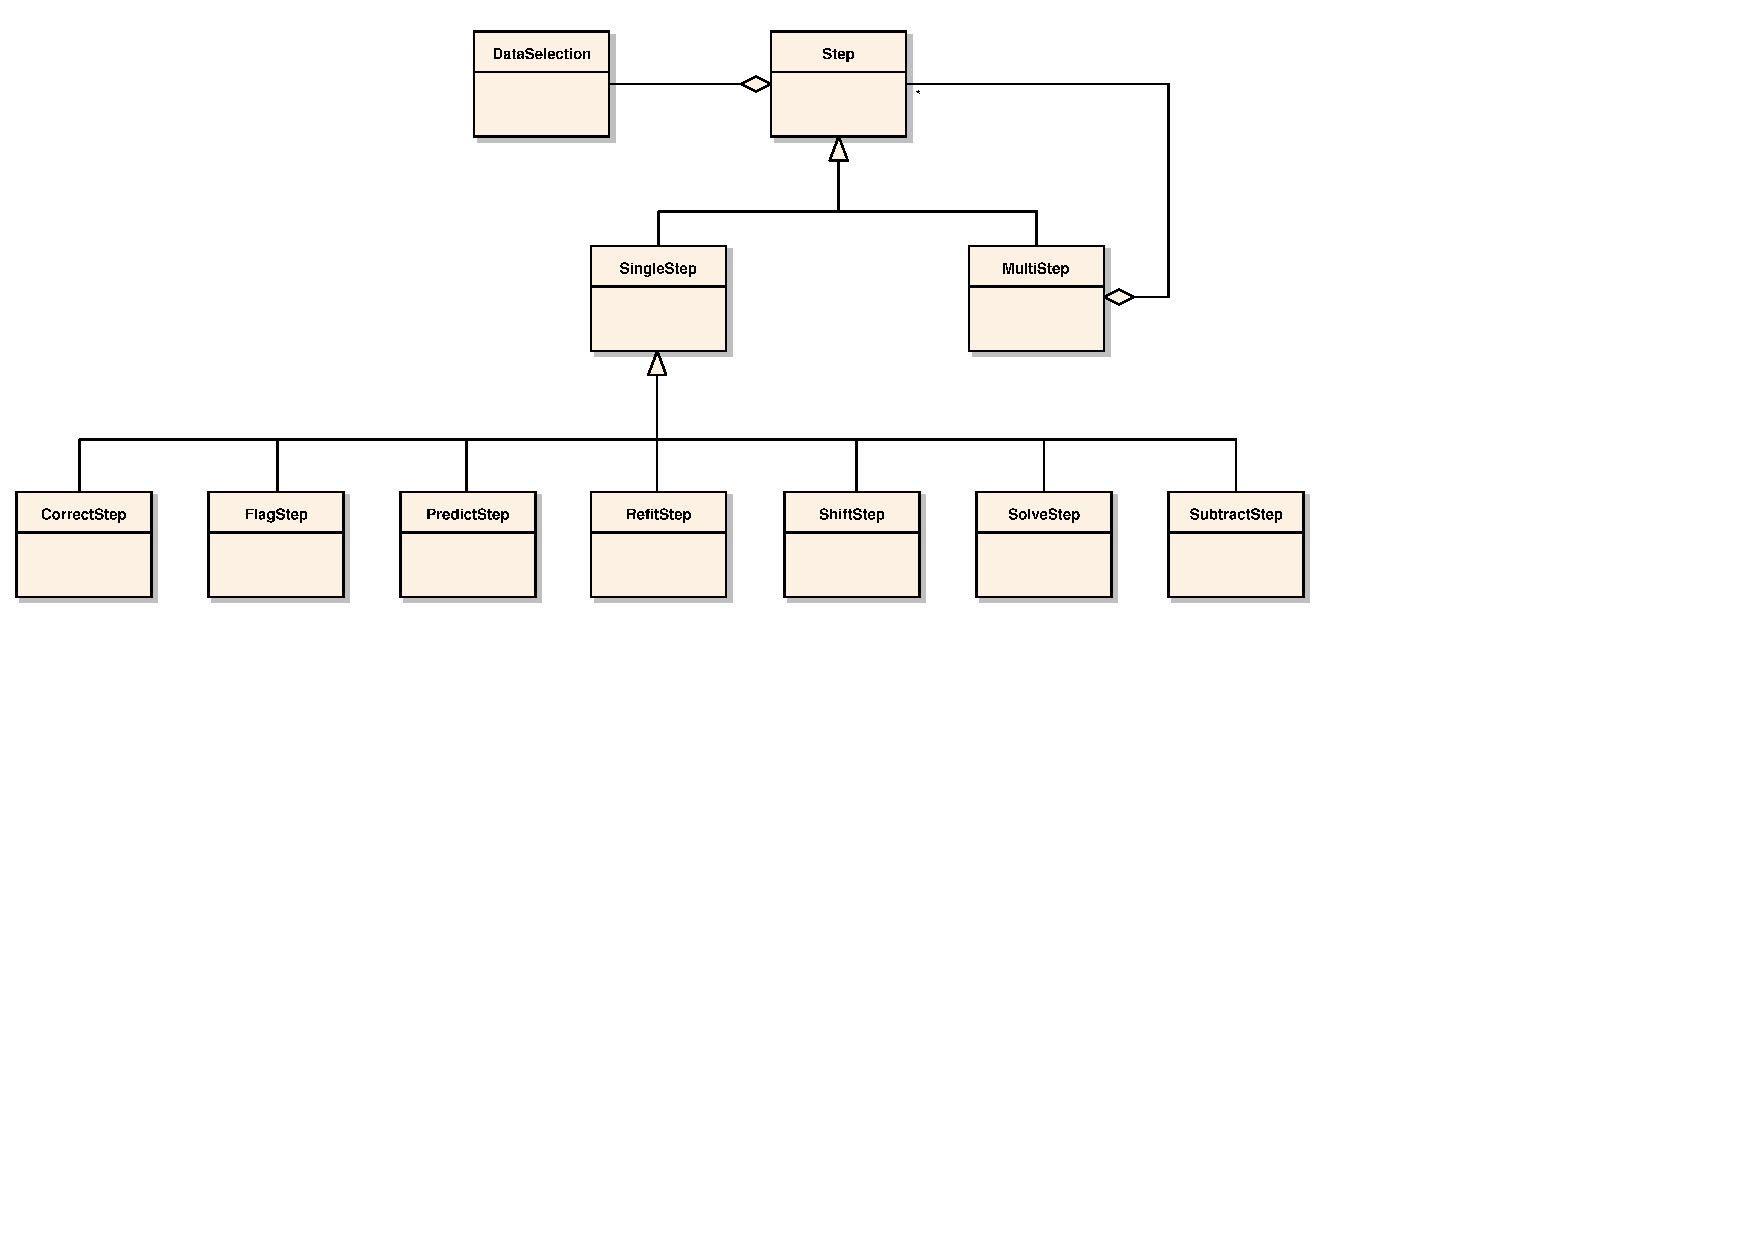
\includegraphics[width=0.8\textwidth]{images/bbs-step-class-diagram}
\caption{The BBS Step class family defines single pieces of work that can be
executed by the BBS Kernel as part of the current self calibration run.}
\label{fig:bbsstep}
\end{figure}

\todo{Remove refit step??}

\subsubsection{Global Control}
\label{subsubsec:design-global-control}
The BBS Global Control is reponsible for managing the execution of a self
calibration run.
\begin{figure}[!ht]
\centering
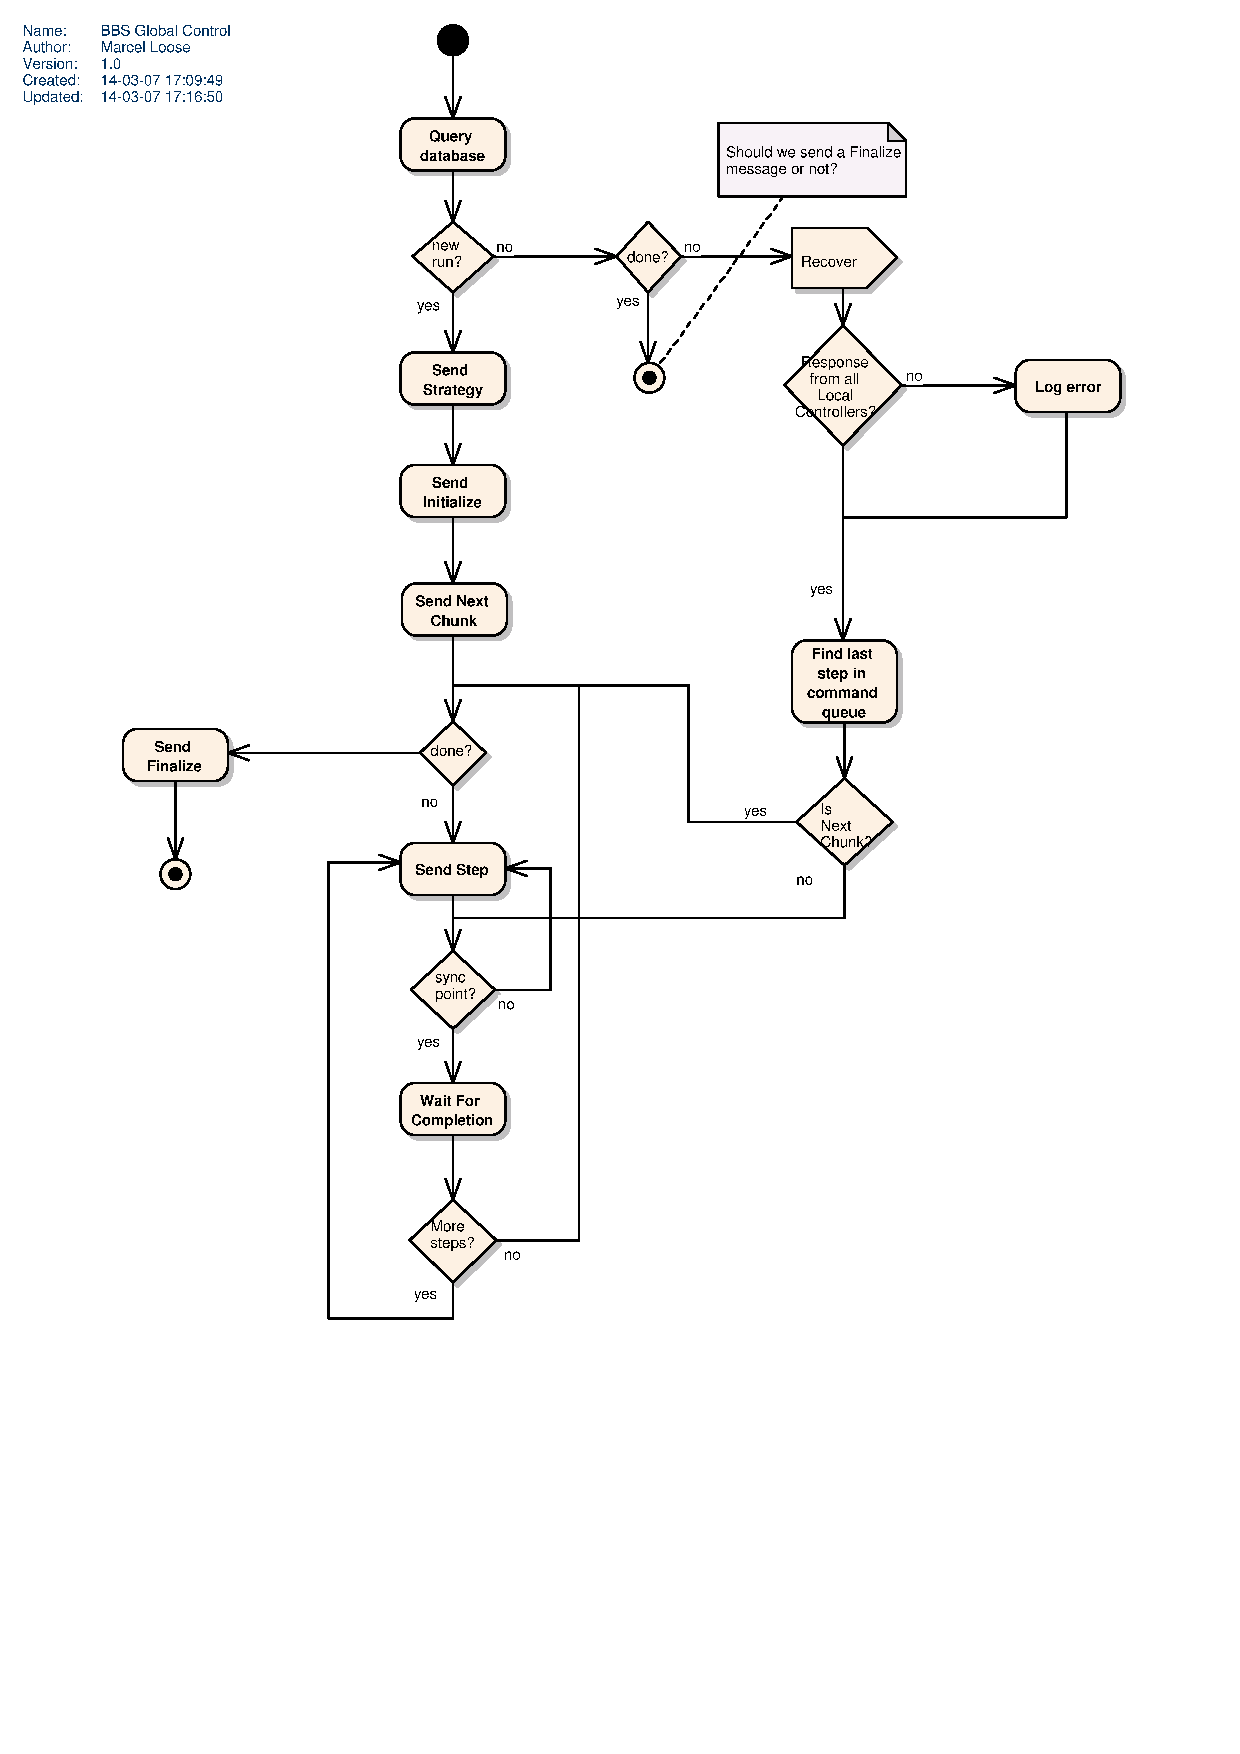
\includegraphics[width=0.7\textwidth]{images/bbs-global-control-activity-diagram}
\caption{Activity diagram of the BBS Global Control}
\label{fig:global-control-activity}
\end{figure}

\subsubsection{Local Control}
\label{subsubsec:design-local-control}
\begin{figure}[!ht]
\centering
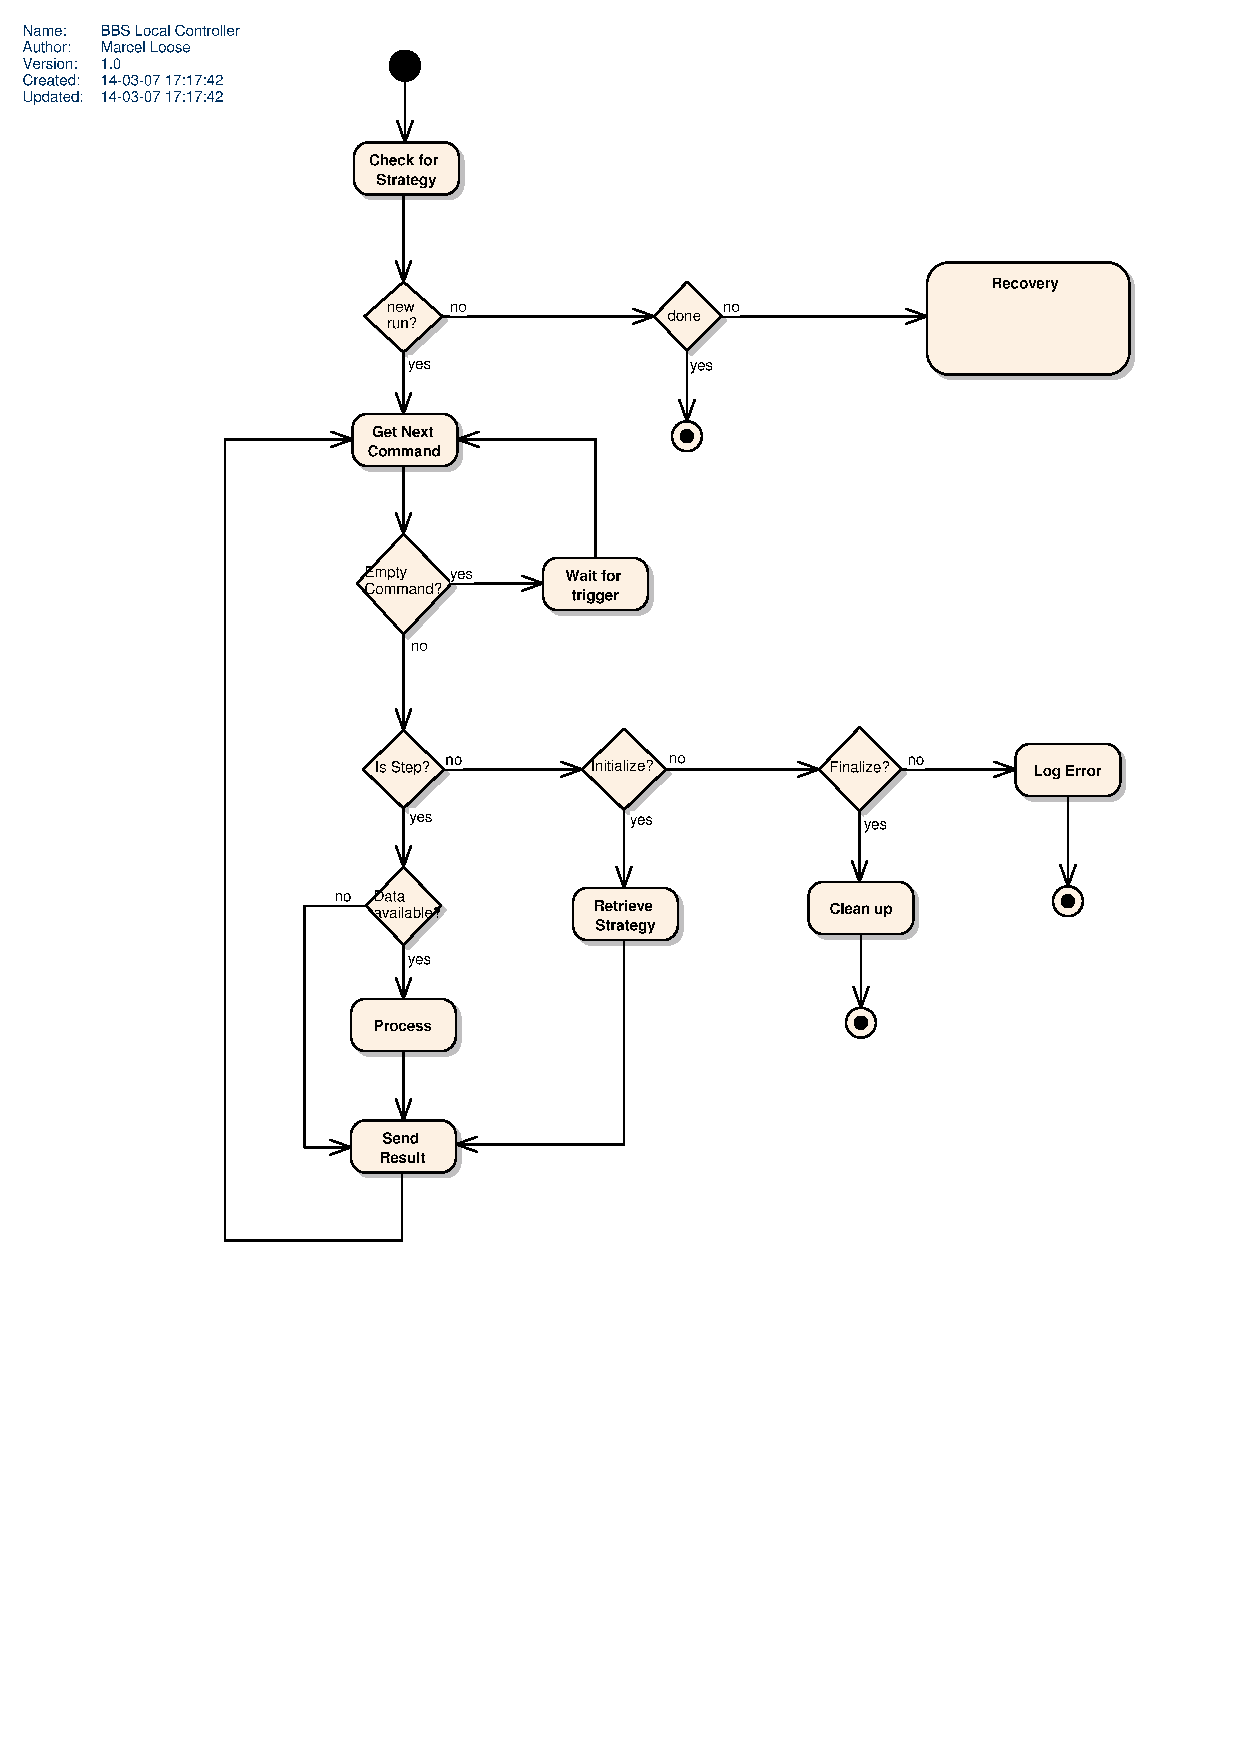
\includegraphics[width=0.7\textwidth]{images/bbs-local-control-activity-diagram}
\caption{Activity diagram of the BBS Local Control}
\label{fig:local-control-activity}
\end{figure}


\subsection{BBS Kernel}
\label{subsec:design-kernel}
The kernel is the part of \bbs responsible for number crunching. It is
implemented as a stand-alone library that is used by the local controller
(BBSKernel executable) and the solver (BBSSolver executable). This simplifies
reuse of kernel code in projects that require a different control
implementation.

\todo{create a simple figure in a more general part of the document that
explains the different packages/libraries/executables/... used in \bbs (see for
example the \olap document)}

The kernel supports four primitive operations:
\begin{itemize}
\item \textsc{predict}\\
Predict (simulate) visibilities based on a model that describes the sky, the
environment (e.g. ionosphere), and the instrument.
\item \textsc{subtract}\\
Predict visibilities for one or more source(s) and subtract the result from the
observed visibilities.
\item \textsc{correct}\\
Correct visibilities for a given reference (source) direction.
\item \textsc{generate equations}\\
Generate condition equations in a form that can be fed to the solver. Condition
equations relate the model parameters to the difference between the observed
visibilities and the predicted visibilities (based on the model).
\end{itemize}

\todo{explain that subtract, generate also include a predict}
\todo{add other steps}

\subsubsection{Measurement Equation Evaluation}
\label{subsubsec:design-me-evaluation}
The Measurement Equation (\me) \cite{LOFAR-ASTRON-ADD-015} is a parameterized
model of an interferometer in terms of a model of the sky, environmental effects
(e.g. ionosphere), and antenna based instrumental effects.

Both \bbs and \meqtree represent the \me as a directed acyclic graph, although
it is commonly referred to as \emph{tree}. The nodes of the tree represent
atomic expressions, while the branches represent dependencies between atomic
expressions. Compound expressions can be build by combining multiple nodes into a
(sub)tree. The leaf nodes represent the parameters of the expression, e.g.
source positions and Stokes vectors. As an example, figure \ref{fig:expr_tree}
shows a subtree for computing the visibilities produced by two linearly
polarized point sources at different positions.
\begin{figure}[htbp]
\centering
\includegraphics[width=\textwidth]{images/expr_graph_sdd.ps}
\caption{This figure shows a subtree for computing the visibilities produced by
two linearly polarized point sources at different positions. The leaf nodes,
i.e. the parameters of the expression, have been colored grey.}
\label{fig:expr_tree}
\end{figure}

\meqtree is very flexible in the expression trees that a user can specify. The
flexibility is due to a powerful Python language extension (\textsc{tdl}) that
allows easy construction of a tree from an arbitrary expression, and to the high
granularity of the nodes. The granularity of the nodes used in \bbs tends to be
lower. For example, in \meqtree a typical node implements the sine function,
whereas in \bbs a single node may implement a bandpass model. Because of the
granularity of the nodes used in \bbs, the expression trees are generally small.
Therefore, the overhead of traversing the trees is small as well. Note that, if
necessary, \bbs could be made more flexible by adding nodes that are less
specialized. By the same reasoning, the overhead of tree traversal in \meqtree
could be reduced by creating specialized nodes.

Specification by the user is limited to selecting predefined subtrees to include
in the \me. Currently implemented subtrees are:
\begin{itemize}
\item Prediction of a (possibly polarized) point source
\item Complex gain per station (G-jones)
\item Complex gain in the direction of a source, per station (E-jones)
\item Bandpass (B-jones)
\end{itemize}

\bbs will automatically generate a complete expression tree based on the
selected predefined subtrees. For example, it will instantiate a subtree for
each selected source in the local sky model and will include these at the
appropriate place in the \me tree for each selected interferometer (baseline).

In \cite[sec. 2]{LOFAR-ASTRON-SDD-050} a more in depth discussion of the various
models, such as beamshape, bandpass, and ionosphere is given. 

\subsubsection{Model Parameters}
To evaluate an expression tree, the kernel needs to know the values of
the model parameters (leaf nodes). Typical examples of model parameters are:
source position and Stokes vector, complex station gain, ionospheric phase
shift. The total number of parameters in the expression trees of the entire
\lofar array will depend on the number of sources that are included in the sky
model. Several thousands of parameters seems to be a realistic estimate
\cite{LOFAR-ASTRON-SDD-052}.

\paragraph{Naming scheme}
Because of the large number of parameters, keeping track of them all becomes a
challenge. A naming scheme can be used to simplify this task. The naming scheme
achieves two goals:
\begin{enumerate}
\item Identification of groups of related parameters
\item Specification of default values
\end{enumerate}

Each parameter is assigned a unique name, which can be made up of several parts
separated by colons. Grouping can be achieved with \textsc{unix}-like wildcards
(*, \{\}), see table \ref{tab:naming_scheme}.
\begin{table}[htb!]
\centering
\begin{tabular}{lp{0.60\textwidth}}
\hline
\textbf{Identifier} & \textbf{Referenced parameter(s)} \\
\hline
\texttt{ra:3C343} & Right ascention of source 3C343 \\
\hline
\texttt{dec:3C343} & Declination of source 3C343 \\
\hline
\texttt{gain:11:phase:CS10:3C343.1} & Phase of the x-polarized signal from
station CS10 in the direction of source 3C343.1 \\
\hline
\texttt{gain:11:phase:*:3C343.1} & Phase of the x-polarized signal of all
stations in the direction of source 3C343.1 \\
\hline
\texttt{gain:\{11,22\}:phase:*:3C343.1} & Phase of both the x- and y-polarized
signal from station CS10 in the direction of source 3C343.1. \\
\hline
\end{tabular}
\caption{Examples of typical parameter names and the use of wildcards to
identify a group of related parameters.}
\label{tab:naming_scheme}
\end{table}
If the kernel cannot find an exact match when searching for a certain parameter,
it will try to find a default value. Default values are specified according to
the same naming scheme as parameters. However, if no default value can be found
that matches the name of a parameter exactly, the kernel will strip off the last
part of the name and retry. This process continues until either a match is found
or the name becomes empty. Thus, one can specify for example a default flux for
every source by specifying \texttt{StokesI}: If the kernel needs the value of
\texttt{StokesI:3C343} but that parameter does not exist as a regular parameter,
it will try to find a default value called \texttt{StokesI:3C343}. If that
default value also does not exist, it will strip off the last part of the name
and search for a default value called \texttt{StokesI}, which does exist in our
example.

\paragraph{Reusing parameter values}
It often makes sense to reuse the parameter values determined during
calibration of an observation $A$ for calibration of an observation $B$. For
instance, to provide a good initial values for the calibration of $B$ and
hopefully save a few iterations.

Instead of straightforward copying of parameter values, interpolation could be
considered. For example, suppose we have already calibrated two observations,
$A$ and $C$, one taken before and one after the time at which the observation to
be calibrated, $B$, was recorded.

Reuse of parameter values can also be applied \emph{during} calibration of an
observation, when moving from one work domain to the next. One could even
consider something like the following algorithm:
\begin{enumerate}
\item Solve a small number of work domains spaced relatively far apart
\item Determine initial values for the intermediate work domains by
interpolation
\item Solve for the intermediate work domains.
\end{enumerate}

\paragraph{Refitting}
Refitting is useful in a multi-resolution approach. A typical scenario would be:
\begin{enumerate}
\item Solve for a parameter using funklets of a low polynomial degree on
relatively large solve domains to get the global trend
\item Refine the solution by using funklets of a higher degree on relatively
small solve domains, using the values found in 1. as a starting point
\end{enumerate}

Funklets are defined on a normalized domain. The normalization depends on the
validity domain. Therefore, the coefficients of funklets defined on a coarse
scale cannot be copied directly to funklets defined on a fine scale. For
polynomials the required transformation is easy to derive. In more complicated
cases, the solver could be used to find the new values.

\todo{Check of bovenstaande juist is.}

\subsubsection{Solving}
\label{subsubsec:design-solver}
\todo{explain that solution can be discontinuous across solve domain boundaries}

\todo{explain that one could solve for scalars and fit afterwards}

%\todo{explain why one doesn't solve for all parameters simultaneously, for one
%big solve domain? (avoid data reload)}

Because each solve domain is \emph{independent} of the other solve domains, the
partitioning of the data domain into solve domains is strongly linked to the
problem of interest. For instance, solving for station gain every \emph{minute}
is a different problem than solving for station gain every \emph{hour}.
BBS can solve for any combination of the parameter coefficients used in the algorithms.

Solvable parameters
In a BBS run it is possible to do a joint solve for any combination of parameters. There is a limitation that the frequency-time domains of the solvable parameters have to be the same.
The number of solvable parameters in a run can vary a lot. For two reasons it should be kept as low as possible:
1.A derivative has to be calculated for each solvable parameter. It means it is better to solve for constant values in small domains than for polynomial coefficients in larger domains. Later it is always possible to fit the constant parameter values to a polynomial (or any other function) on a larger domain.
2.Inverting the solver matrix is a $O(N^3)$ problem. As the size of the fitter matrix is determined by the number of solvable parameters, it is clear that the number should be kept as low as possible.
It means that it makes no sense to combine multiple domains in a single solve, because each domain has its own set of parameter values.

Some examples of parameters to solve are:
Ionospheric phases for a patch in the sky require 74 parameters per patch (for 37 stations).
To keep the number of parameters low it is best to solve patch by patch. In  it is argued that this approach is also best in peeling the visibility onion.
Point source fluxes and/or positions require 1-6 parameters per source assuming that no polynomial or so is used to represent the fluxes.


It follows that solving for $0^{th}$-degree funklets using one channel width times one integration period solve domains is equivalent to solving for a sampled version of the parameter value. A larger solve domain may be used to increase the signal to noise, or to get enough condition equations when solving for multiple parameters simultaneously. From a practical point of view, a large solve/validity domain also decreases the number of parameter values that need to be stored. Storing a set of funklet coefficients per visibility will most likely require too much storage space.

\todo{Klopt de bovenstaande alinea en is ie duidelijk genoeg?}

An important consequence of using funklets is that, given a polynomial degree $n$ and irrespective of the size of the validity domain, it is implicitly assumed that the parameter value is well approximated by a $n^{th}$-degree polynomial on the validity domain. To make this assumption more explicit, it may be useful to interpret the $n^{th}$-degree polynomial as a model, instead of an integral part of parameter handling.

%\subsubsection{Local solver}
%\label{subsubsec:local-solver}
In the design of \textsc{bbs}\begin{footnotesize}3\end{footnotesize}, only a
single global solver was foreseen. This implies the normal equations of all
solve domains were sent to the global solver, even if some of these solve
domains were entirely local to a node. Therefore, it was decided to introduce a
local solver at each node as part of the \cs{1} milestone. Solve domains that
are entirely local can then be solved by the local solver, avoiding
communication overhead and unnecessary synchronization.

We intend to use one implementation for both local and global solver. On each
node a separate solver process will be started. The normal equations for
entirely local solve domains will be sent to the solver process running on the
same node. For solve domains that span several nodes, a separate pool of global
solvers could be used or the solver process at one of the involved nodes could
be designated to act as global solver.

Each of the nodes will sent its normal equations to the designated solver.
Communication will be performed via sockets. If performance turns out to be
poor, we can always re-integrate the local solver and the prediffer. This avoids
the memory and communication overhead of sending the normal equations for
entirely local solve domains over a (unix domain) socket.


\subsection{BBS Database}
\label{subsec:design-database}

The current Prediffer implementation can handle parameters as follows:
At the first iteration it reads the parameters from an NFS-visible Berkeley DB (BDB) database or AIPS++ table.
The Prediffer can handle the updated parameter values in 3 ways:
Read from an NFS-visible database or AIPS++ table.
Read from a replicated BDB database.
Receive from the Controller.
Given the amount of parameters and domains, searching parameters and domains in
the database can take some time. Optimization of the parameter data structure
and evaluation of high-performance distributed embedded databases are ongoing.

\subsubsection{Data Model}
\label{subsubsec:design-data-model}
%\begin{figure}[!ht]
%\includegraphics[width=\textwidth]{images/blackboard-datamodel}
%\caption{Data model of the Blackboard database}
%\end{figure}

\subsubsection{Work Orders}
\label{subsubsec:design-work-orders}

\subsubsection{Parameter Solutions}
\label{subsubsec:design-parmsolutions}

\subsection{Performance considerations}
\label{subsec:performance-considerations}

\subsubsection{Double vs. single precision}
\subsubsection{Other vis. format / mmap}
Currently mmap is used to read and write the data in the MeasurementSet. Although it works fast and nice, it has the problem that it makes it impossible to use a large work domain where data are selected and/or integrated. It also makes it hard to use a MeasurementSet containing tiled data.
It would be better to have a separate IO thread (or process) that can read, write, select, and integrate the data asynchronously and transports the data as MeqMatrix objects.

The description of each MeasurementSet is currently stored in a blob in a .des file. It would be better to let the IO thread retrieve that info from the MeasurementSet and send it as a blob to the Prediffers.

\todo{Possibility of mistakes is also large!}


\subsubsection{Parameter spatial queries}
\subsubsection{Process / code level parallelism}
Apart from the distributed processing described before, the BBS system also exploits parallelization in the Prediffers as much as possible. This form of parallelization is for nodes with multiple CPUs and CPU-cores which are both envisaged in the CEP implementation. This parallelization is done by using multi-threading in the calculation of the result of the expression tree. Because a node in the tree can be used by multiple parents, a straightforward parallel execution of the tree is not possible. Instead the tree is analyzed to find the dependency level of each node. Starting at the lowest level the nodes at each level are calculated in parallel and the results are cached. In this way all calculations can be done in parallel without the need of explicit locking and waiting.

Because most calculations are done for a vector of frequencies, it is possible to use vectorized instructions on modern processors. A special code generator has been developed to assist in using SSE2 instructions for this purpose.

\subsubsection{Minimisation}
\begin{itemize}
\item Joint solving (SDD-052, page 19)
\item Solvable parameter count (SDD-052. page 16)
\end{itemize}

In a BBS run it is possible to do a joint solve for any combination of parameters. There is a limitation that the frequency-time domains of the solvable parameters have to be the same.
The number of solvable parameters in a run can vary a lot. For two reasons it should be kept as low as possible:
1.A derivative has to be calculated for each solvable parameter. It means it is better to solve for constant values in small domains than for polynomial coefficients in larger domains. Later it is always possible to fit the constant parameter values to a polynomial (or any other function) on a larger domain.
2.Inverting the solver matrix is a $O(N^3)$ problem. As the size of the fitter matrix is determined by the number of solvable parameters, it is clear that the number should be kept as low as possible.
It means that it makes no sense to combine multiple domains in a single solve, because each domain has its own set of parameter values.
Some examples of parameters to solve are:
Ionospheric phases for a patch in the sky require 74 parameters per patch (for 37 stations).
To keep the number of parameters low it is best to solve patch by patch. In  it is argued that this approach is also best in peeling the visibility onion.
Point source fluxes and/or positions require 1-6 parameters per source assuming that no polynomial or so is used to represent the fluxes.


\subsubsection{Data handling/caching}
\todo{Move disussion about this subject to more global document?}

\subsubsection{Parameter database access / central database}
Prediffers look in the BlackBoard Database for new work orders. The load on the
database can be very high if many processes are polling it to look for work
orders. It might be better to turn the BlackBoard into a process or to send the
work orders directly from the controller to the Solver and Prediffer processes.
A database can still be used as a logging mechanism and for monitoring by
external processes.

\begin{itemize}
\item Asynchronous notification
\item Do not store intermediate results? (solve history)
\end{itemize}


\cleardoublepage

% References
\bibliographystyle{unsrt}
\bibliography{lofar}

\cleardoublepage

\appendix
\section{Configuration Syntax}

This appendix describes the syntax of the BBS configuration file (a.k.a.
parset). Its goal is to foster a common understanding and terminology. At the
moment this page is still under construction. I've added
\textcolor{red}{questions in red} to things that were not clear to me while
creating this page. Thing to do are \textcolor{green}{stated in green}.

\subsection*{Global Settings}
\begin{description}
\item [DataSet] : \emph{string} \\
    Path to the input measurement set.
\item [BBDB] : \emph{BBDB} (see page \pageref{app-bbdb}) \\
    Information about the black board database.
\item [ParmDB] : \emph{ParmDB} (see page \pageref{app-parmdb}) \\
    Information about the parameter databases (e.g. instrument parameters,
    local sky model).
\end{description}

\subsubsection*{Example}
{\footnotesize
\begin{verbatim}
DataSet                  = "test.ms"    # name of Measurement Set

BBDB.Host                = "127.0.0.1"  # hostname/ipaddr of BB DBMS
BBDB.Port                = 12345        # port used by BB DBMS
BBDB.DBName              = "blackboard" # name of the BB database
BBDB.UserName            = "postgres"   # username for accessing the DBMS
BBDB.PassWord            = ""           # password for accessing the DBMS

ParmDB.Instrument        = "test.mep"   # instrument parameters (MS table)
ParmDB.LocalSky          = "test.gsm"   # local sky parameters (MS table)
\end{verbatim}
}

\subsection*{Strategy}
A strategy consists of one or more (multi-)steps with an associated work domain
size and optional data integration.
\begin{description}
\item [Steps] : \emph{vector$<$string$>$} \\
    The names of the steps that compose the strategy. It is an error to leave
    this field empty.
\item [Stations] : \emph{vector$<$string$>$} \\
    Names of the participating stations. All stations will be used if this
    field is left empty.
\item [InputData] : \emph{string} \\
    Name of the column in the measurement set that contains the input data.
\item [Correlation] : \emph{Correlation} (see page \pageref{app-correlation}) \\
    Specifies which correlations to use.
\item [WorkDomainSize] : \emph{DomainSize} (see page \pageref{app-domainsize}) \\
    Size of the work domain in frequency and time. A work domain represents an
    amount of input data that is loaded into memory and processed as a single
    block.  A large work domain size should reduce the overhead due to disk
    access.
\item [Integration] : \emph{DomainSize} (see page \pageref{app-domainsize}) \\
    Cell size for integration. Allows the user to perform operations on a
    lower resolution, which should be faster in most cases.
\end{description}

\subsubsection*{Example}
{\footnotesize
\begin{verbatim}
Strategy.Steps                 = ["MultiStep", "SingleStep2"] \
                                                # (multi-)steps that compose this strategy
Strategy.Stations              = [ 0, 1, 2, 3 ] # ID's of stations to use
Strategy.InputData             = "INDATA"       # MS input data column
Strategy.Correlation.Selection = ALL            # one of AUTO, CROSS, ALL
Strategy.Correlation.Type      = ["XX", "YY"]   # which (cross)correlations to use
Strategy.WorkDomainSize.Freq   = 1e+6           # work domain size: f(Hz)
Strategy.WorkDomainSize.Time   = 10             # work domain size: t(s)
Strategy.Integration.Freq      = 1              # integration interval: f(Hz)
Strategy.Integration.Time      = 0.1            # integration interval: t(s)
\end{verbatim}
}

\subsection*{Step}
A \emph{single-step} describes one unit of work of the strategy. A step that
is defined in terms of a number of other steps is known as a multi-step. The
attributes of a \emph{multi-step} should be interpreted as default values for
the steps that compose the multi-step. These default values can always be
overridden.
\begin{description}
\item [Steps] : \emph{vector$<$string$>$} \\
    The names of the steps that compose this step (for multi-steps), or absent
    (for single steps).
\item [Baselines] : \emph{Baselines} (see page \pageref{app-baselines}) \\
    Baselines to use.
\item [Sources] : \emph{vector$<$string$>$} \\
    Sources to use. All sources will be used if this field is left empty.
\item [ExtraSources] : \emph{vector$<$string$>$} \\
    Additional sources to include when predicting visibilities. If this field
    is left empty, no extra sources will be included.
\item [Correlation] : \emph{Correlation}  (see page \pageref{app-correlation}) \\
    Specifies which correlations to use.
\item [Integration] : \emph{DomainSize}  (see page \pageref{app-domainsize}) \\
    Cell size for integration. Allows the user to perform operations on a
    lower resolution, which should be faster in most cases.
\item [InstrumentModel] : \emph{vector$<$string$>$} \\
    The parts of the measurement equation that should be included. \par
    \textcolor{green}{TODO: add descriptions for the various parts of the ME.}
\item [Operation] : \emph{string} \\
    The operation to be performed in this step. One of SOLVE, SUBTRACT,
    CORRECT, PREDICT, SHIFT, or REFIT. Only relevant for single steps, should
    be absent for multi-steps. \par\
    SOLVE : Find values for the parameters that minimize the difference
    between the predicted and the measured (u,v) values. \par
    \textcolor{green}{TODO: add descriptions for other values.}
\item [OutputData] : \emph{string} \\
    Column in the measurement set wherein the output values of this step
    should be written. If left empty, no data will be written.
\end{description}

\emph{Single steps should define one of the following fields, depending on the
value of \textbf{Operation}} :
\begin{description}
\item [Solve] : \emph{Solve} (see page \pageref{app-solve}) \\
    Arguments of the SOLVE operation. \par
    \textcolor{green}{TODO: specify arguments for the other operations.}
\end{description}

\subsubsection*{Example}
{\footnotesize
\begin{verbatim}
Step.MultiStep.Steps                   = ["SingleStep1", "SingleStep2"] \
                                                                   # steps that compose this multi-step
Step.MultiStep.Baselines.Station1      = [0, 0, 0, 1, 1, 2]        # baselines to use
Step.MultiStep.Baselines.Station2      = [0, 1, 2, 1, 2, 2]        # (all if empty)
Step.MultiStep.Sources                 = ["3C343"]                 # list of sources
Step.MultiStep.ExtraSources            = ["M81"]                   # list of sources outside patch
Step.MultiStep.InstrumentModel         = ["BANDPASS", "TOTALGAIN", "PATCHGAIN"] \ 
                                                                   # instrument model
Step.MultiStep.Integration.Freq        = 2                         # integration interval: f(Hz)
Step.MultiStep.Integration.Time        = 0.5                       # integration interval: t(s)
Step.MultiStep.Correlation.Selection   = CROSS                     # one of AUTO, CROSS, ALL
Step.MultiStep.Correlation.Type        = ["XX", "XY", "YX", "YY"]  # which (cross) correlations to use

Step.SingleStep1.Baselines.Station1    = [0, 1]                    # baselines to use
Step.SingleStep1.Baselines.Station2    = [1, 2]                    # (all if empty)
Step.SingleStep1.Sources               = []                        # list of sources
Step.SingleStep1.InstrumentModel       = ["BANDPASS", "TOTALGAIN"] # instrument model
Step.SingleStep1.Operation             = SOLVE                     # one of SOLVE, SUBTRACT, CORRECT, \
                                                                   # PREDICT, SHIFT, REFIT
Step.SingleStep1.OutputData            = "OUTDATA1"                # MS output data column
Step.SingleStep1.Solve.MaxIter         = 10                        # maximum number of iterations
Step.SingleStep1.Solve.Epsilon         = 1e-7                      # convergence threshold
Step.SingleStep1.Solve.MinConverged    = 0.95                      # fraction that must have converged
Step.SingleStep1.Solve.Parms           = ["PHASE:*"]               # names of solvable parameters
Step.SingleStep1.Solve.ExclParms       = [""]                      # parameters excluded from solve
Step.SingleStep1.Solve.DomainSize.Freq = 1000                      # f(Hz)
Step.SingleStep1.Solve.DomainSize.Time = 1                         # t(s)

Step.SingleStep2.Baselines.Station1    = []                        # baselines to use
Step.SingleStep2.Baselines.Station2    = []                        # (all if empty)
Step.SingleStep2.Sources               = []                        # list of sources
Step.SingleStep2.InstrumentModel       = ["DirGain", "Phase"]      # instrument model
Step.SingleStep2.Operation             = CORRECT                   # one of SOLVE, SUBTRACT, CORRECT, \
                                                                   # PREDICT, SHIFT, REFIT
Step.SingleStep2.OutputData            = "OUTDATA2"                # MS output data column
\end{verbatim}
}

\subsection*{BBDB}
\label{app-bbdb}
This contains information on how the blackboard database and the parameter
databases can be reached.
\begin{description}
\item [Host] : \emph{string} \\
    Hostname or IP address of the host on which the black board database and
    the parameter databases reside.
\item [Port] : \emph{int} \\
    Port number on which the blackboard database server is listening.
\item [DBName] : \emph{string} \\
    Name of the black board database.
\item [UserName] : \emph{string} \\
    Username to access the black board database.
\item [PassWord] : \emph{string} \\
    Password to access the black board database.
\end{description}

\subsection*{ParmDB}
\label{app-parmdb}
\begin{description}
\item [Instrument] : \emph{string} \\
    Path to the AIPS++ table containing the instrument parameters.
\item [LocalSky] : \emph{string} \\
    Path to the AIPS++ table containing the local sky model parameters.
\item [History] : \emph{string}
    Path to the AIPS++ table containing the solve history.
\end{description}

\subsection*{Correlation}
\label{app-correlation}
\begin{description}
\item [Selection] : \emph{string} \\
    Station correlations to use. Should be one of 'AUTO', 'CROSS', or 'ALL'.
    \par
    AUTO: Use only correlations of each station with itself (i.e. no base
    lines). \textcolor{red}{Not yet implemented.} \\ CROSS: Use only
    correlations between stations (i.e. base lines). \\ ALL: Use auto and
    cross correlations both.
\item [Type] : \emph{string} \\
    Correlations of which polarizations to use, one or more of 'XX', 'XY',
    'YX', 'YY'. As an example, suppose we select 'XX' here and set Selection
    to 'AUTO', then the X polarization signal of each station is correlated
    with itself.  However, if we set Selection to 'CROSS' then the X
    polarization of station A is correlated with the X polarization of station
    B for each base line (A,B)
\end{description}

\subsection*{DomainSize}
\label{app-domainsize}
\begin{description}
\item [Freq] : \emph{double} \\
    The size of the domain in frequency (Hz).
\item [Time] : \emph{double} \\
    The size of the domain in time (s).
\end{description}

\subsection*{Baselines}
\label{app-baselines}
The selected baselines. A baseline is a pair of stations. The first station of
the pair is contained in Station1, the second in Station2. For example,
suppose we have six baselines: (A, B), (A, C), (A, D), (B, C), (B, D), (C,
D). Then Station1 would contain [A, A, A, B, B, C] and Station2 would contain
[B, C, D, C, D, D]. The lengths of Station1 and Station2 should always be
equal. If both fields are left empty, all baselines are used.
\begin{description}
\item [Station1] : \emph{vector$<$string$>$} \\
    One name for each baseline: the first station in the pair that forms the
    baseline.
\item [Station2] : \emph{vector$<$string$>$} \\
    One name for each baseline: the second station in the pair that forms the
    baseline.
\end{description}

\subsection*{Solve}
\label{app-solve}
\begin{description}
\item [MaxIter] : \emph{int} \\
    Maximum number of iterations.
\item [Epsilon] : \emph{double} \\
    Minimal difference between the old and the new parameter values after each
    iteration. When the difference falls below this threshold, the solver will
    stop iterating.
\item [MinConverged] : \emph{double} \\
    Minimal fraction of solve domains that must have converged to declare
    overall convergence.
\item [Parms] : \emph{vector$<$string$>$} \\
    Parameters to solve for. Wildcards are allowed, e.g. BANDPASS:*.
\item [ExclParms] : \emph{vector$<$string$>$} \\
    Subset of the parameters selected by Parms that should not be solved for.
    For example, if we would like to solve for the gain (amplitude, phase) of
    each station, but we would also like to fix the phase of the first station
    (STATION0) this can be specified as follows: {\footnotesize
\begin{verbatim}
Solve.Parms = ["gain:*"]
Solve.ExclParms = ["gain:*:phase:STATION0"]
\end{verbatim}
}
\item [DomainSize] : \emph{DomainSize} \\
    Size of the solve domain. The work domain is divided in solve domains and
    a solution is computed for each solve domain independently.
\end{description}



\end{document}
